\chapter{การออกแบบและระเบียบวิธีวิจัย}

\section{ภาพรวมของระบบ}

บทนี้จะกล่าวถึงภาพรวมของระบบโดยแสดงเป็นไดอะแกรมดังรูปที่ \ref{fig:systemoverview} ซึ่งประกอบไปด้วยการออกแบบระบบฐานข้อมูล ระบบการตัดคำ ระบบการประมวลรูปภาพ และการออกแบบ User Interface สำหรับการใช้งาน

\begin{figure}[H]
    \centering
    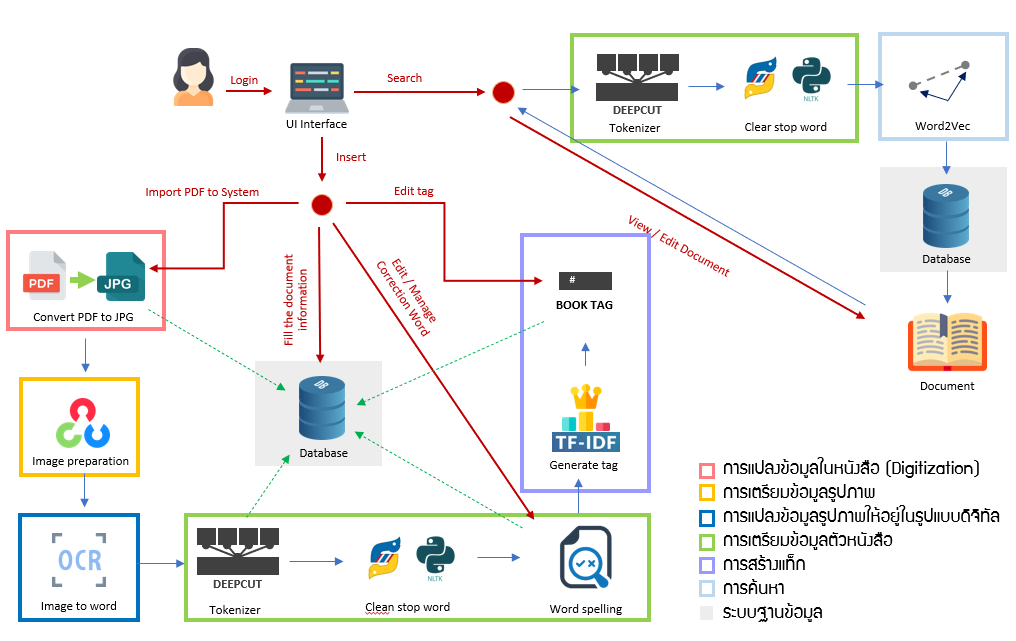
\includegraphics{systemoverview}
    \caption{ภาพรวมของระบบ}\label{fig:systemoverview}
\end{figure}

\section{การออกแบบการทดลอง}
\subsection{การแปลงหนังสือเป็นรูปภาพ}

สำหรับการแปลงหนังสือผู้ใช้จะต้องทำการอัปโหลดไฟล์ PDF ของหนังสือเข้าสู่ระบบหลังจากนั้นจะระบบจะทำการแปลงแต่ละหน้าเป็นรูปภาพ JPG เพื่อนำไปใช้ต่อในขั้นต่อไปและนำใช้แสดงภายใน web application

\subsection{การเตรียมข้อมูลรูปภาพ}

ในส่วนของการจัดการรูปก่อนที่จะทำการ OCR ซึ่งรูปภาพนำมา OCR นั้นมาจากการสแกนทำให้ภาพส่วนใหญ่อยู่ในสภาพดีแต่ก็ยังคงมี noise  และมีความผิดพลาดจากการสแกนเช่น ภาพเอียง หรือตัวหนังสือไม่ชัดเกิดจากการขยับในระหว่างการสแกน หรือมีพื้นหลังสีที่ทำให้ OCR ไม่มีประสิทธิภาพ ดังนั้นจึงต้องมีการเตรียมข้อมูลรูปภาพก่อนที่จะไปทำ OCR
ซึ่งในการเตรียมข้อมูลรูปภาพ นั้นทางคณะผู้จัดทำได้ออกแบบไว้ว่าจะทำการแยกระหว่างรูปและตัวหนังสือออกจากกัน โดยการใช้คอนทัว(contour) เข้ามาช่วยในการคัดแยกรูปออกจากตัวอักษร โดยดูจากพื้นที่สี่เหลี่ยมที่ของคอนทัว(contour) กับพื้นที่คอนทัว(contour) ว่ามีความต่างขนาดและความแตกต่างกันมากเท่าไร หรือใช้ขนาดความกว้างและยาวมาดูว่ามีขนาดเกินเท่าไรถึงจะตัดให้เป็นรูปภาพ
นอกจากนี้ออกแบบการหมุนโดยสร้างคอนทัว(contour) บรรทัดและวัดความเอียงของแต่ละบรรทัดว่าเอียงเท่าไรจากนั้นจึงหมุนกลับในองศาตรงข้าม


\subsubsection{การข้ามหน้า}

โดยการทำการคัดหน้าสีนั้น เราได้นำค่าความถี่ของหน้าที่มีพื้นหลังสีมาพล็อตเพื่อหาความแตกต่างจะเห็นได้ว่าถ้าหน้าที่มีพื้นหลังสี หลายสีนั้นจะมีค่าความถี่กระจายอยู่หลายค่าในขณะที่ถ้าเป็นหน้าที่มีพื้นหลังสีเดียวมีค่าความถี่ในช่วงนั้นสูงดังรูป \ref{fig:skippage}

\begin{figure}[H]
    \centering
    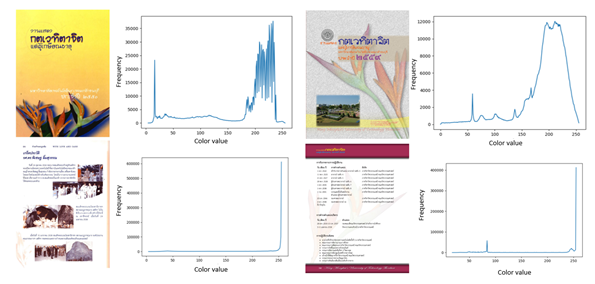
\includegraphics[scale=0.8]{skippage2}
    \caption{ภาพแสดงความถี่ของภาพพื้นหลังสีและภาพพื้นหลังขาวดำ}\label{fig:skippage2}
\end{figure}

\underline{ขั้นตอนหลักการทำงานของการข้ามหน้า}

\begin{enumerate}
    \item รับไฟล์รูปภาพมาแปลงเป็น Gray Scale และทำการปรับตัวแปรที่เป็นรูปภาพแบบ Gray Scale ให้เป็นอาเรย์มิติเดียว
    \item ทำการนับความถี่ของค่าสีว่าแต่ละค่าสีนั้นมีจำนวนเท่าไหร่
    \item นำค่าความถี่ของค่าสีที่มีความถี่สูงสุดมาคำนวณว่ามีค่ามากกว่า 10 เปอร์เซ็นต์ของจำนวนพิกเซลทั้งหมดหรือไม่ ถ้าน้อยกว่าให้ข้ามการทำ OCR หน้านี้ไป
\end{enumerate}

\begin{figure}[H]
    \centering
    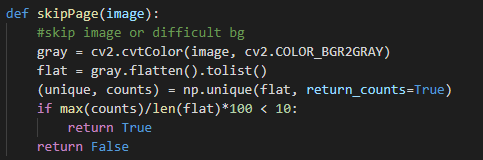
\includegraphics[scale=0.8]{skippage}
    \caption{ภาพแสดงขั้นตอนการข้ามหน้า}\label{fig:skippage}
\end{figure}

\subsubsection{การหมุนรูป}

โดยจะมีหลักการหมุนด้วยวิธีการหาค่าองศาของแต่ละประโยคด้วยวิธีการนำจุด 2 ที่อยู่ในแนวระราบเดียวกันมาทำการหา arctan เพื่อหาองศาที่ทำให้บรรทัดนั้นตรง และนำค่าองศาแต่ละบรรทัดที่อยู่ในย่อหน้าเดียวกันมาหาองศาเฉลี่ยเพื่อที่จะใช้การหมุนทั้งย่อหน้าให้ตรง

\underline{ขั้นตอนการหมุน}

\begin{enumerate}
    \item เริ่มจากนำรูปภาพมาทำเป็นสองส่วนคือการทำขยายภาพ(dilate) และกร่อนภาพ(erode) โดยที่รูปภาพที่ถูกขยายจะได้รูปที่มีการจับกลุ่มบรรทัดของย่อหน้า และรูปที่ถูกกร่อนจะได้รูปภาพที่มีการแยกบรรทัดข้อความกันอย่างชัดเจน และนำไปหาคอนทัว(contour) โดยที่รูปภาพของการจับกลุ่มบรรทัดจะได้ผลลัพธ์ดังรูปภาพที่ \ref{fig:rotate2} ทางด้านซ้าย และการแยกบรรทัดจะได้ผลลัพธ์ดังรูปภาพที่ \ref{fig:rotate2} ทางด้านขวา 
    
    \begin{figure}[H]
        \centering
        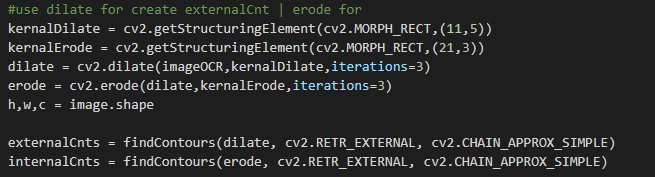
\includegraphics[scale=0.8]{rotate1}
        \caption{ภาพแสดงการทำการกร่อนภาพ(erosion) และการขยายภาพ(dilation)}\label{fig:rotate1}
    \end{figure}
    
    \begin{figure}[H]
        \centering
        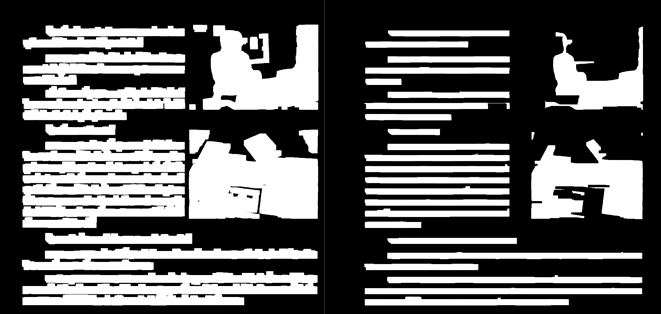
\includegraphics[scale=0.8]{rotate2}
        \caption{ภาพแสดงการเปรียบเทียบการทำการกร่อนภาพ(erosion) และการขยายภาพ(dilation)}\label{fig:rotate2}
    \end{figure}

    \item ทำการแยก รูปภาพและบรรทัดข้อความ ภายในคอนทัว(contour)ที่ถูกกร่อน โดยการกำหนดค่าความสูงสูงที่สุดและต่ำที่สุดไว้ ค่าอัตราส่วนระหว่างความสูงและความกว้าง โดยค่าที่กำหนดไว้เราได้เอามาจากการทำ Page dewarp ของ Matt Zucker \cite{mattzuck} และนำมาตรวจสอบเงื่อนไขและแยกเป็นกลุ่มของข้อความและรูปภาพดังรูปภาพที่ \ref{fig:rotate3}
    
    \begin{figure}[H]
        \centering
        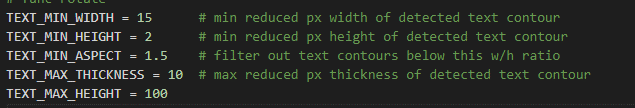
\includegraphics[scale=0.8]{rotate3}
        \caption{ภาพแสดงเกณฑ์การวัดบรรทัดของตัวหนังสือ}\label{fig:rotate3}
    \end{figure}
    
    \begin{figure}[H]
        \centering
        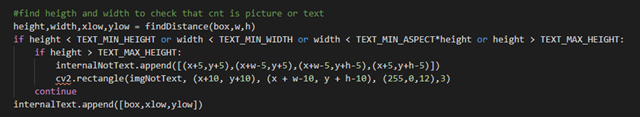
\includegraphics[scale=0.8]{rotate4}
        \caption{ภาพแสดงการคัดแยกคอนทัว(contour) ที่ไม่ใช่ตัวหนังสือ}\label{fig:rotate4}
    \end{figure}

    \item ทำการหา Mask เพื่อใช้ในการลบรูปภาพและคำนวณองศาของแต่ละบรรทัดข้อความภายในคอนทัว(contour)ของภาพที่ถูกขยาย(dilate)นั้น โดยการลบรูปภาพจะทำโดยการระบุว่ารูปภาพอยู่ว่าภายในคอนทัว(contour) ที่ถูก ไหนเพื่อจะนำมาเป็น mask สำหรับการลบรูปภาพออกด้วยวิธีการดูว่าคอนทัว(contour) ที่ถูกแยกเป็นรูปภาพนั้นอยู่ภายในคอนทัว(contour)ภาพที่ถูกขยาย(dilate) ครบทั้งสี่มุมหรือเปล่า ถ้าใช่แสดงว่าคอนทัว(contour)ภาพที่ถูกขยาย(dilate) คือ mask ของรูปภาพที่จะต้องถูกลบให้สร้างคอนทัว(contour)ภาพที่ถูกขยาย(dilate)นั้นลงไปบนรูปแต่ถ้าไม่ใช่ก็จะนำไปหาองศาของแต่บรรทัดข้อความและนำมาเฉลี่ยเป็นองศาที่ต้องหมุนสำหรับคอนทัว(contour)ภาพที่ถูกขยาย(dilate) นั้น
    
    \begin{figure}[H]
        \centering
        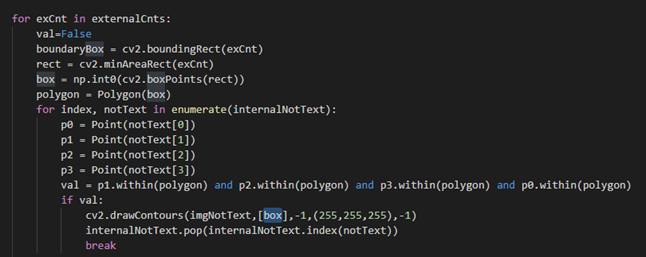
\includegraphics[scale=0.8]{rotate5}
        \caption{ภาพแสดงการทำ Mask ในส่วนที่ไม่ใช่ตัวหนังสือ}\label{fig:rotate5}
    \end{figure}

    \begin{figure}[H]
        \centering
        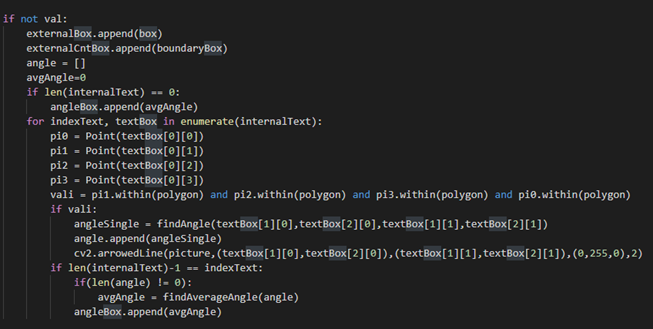
\includegraphics[scale=0.8]{rotate6}
        \caption{ภาพแสดงการคัดตัวหนังสือเพื่อนำไปหาองศาในการหมุน}\label{fig:rotate6}
    \end{figure}

    \begin{figure}[H]
        \centering
        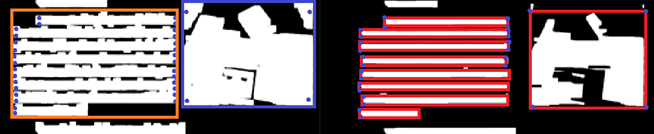
\includegraphics[scale=0.8]{rotate7}
        \caption{ภาพแสดงการจุดของคอนทัว(contour) เล็กในคอนทัว(contour)ใหญ่}\label{fig:rotate7}
    \end{figure}

    \item นำ Mask ที่เป็นรูปภาพนำมาลบออกโดยเมื่อได้ mask มาก็จะนำไปลบออกจากรูปใหญ่ในฟังก์ชั่น removePicture ในรูปที่ \ref{fig:rotate8}  ซึ่งจะนำเอาคอนทัว(contour)ภาพที่ถูกขยาย(dilate) ที่เป็นตัวหนังสือ (กรอบสีเขียว) มาลบออกจาก mask เดิม(กรอบสีแดง)ที่ได้สร้างไว้เพื่อกันการลบพื้นที่เป็นตัวหนังสือดัง \ref{fig:rotate9} ด้วยการใช้ฟังก์ชั่น drawContour ก่อนจะนำ mask ที่ได้มาลบรูปออกทำให้ภาพในแต่ละหน้าหายไป เป็นผลลัพธ์ออกมาดัง \ref{fig:rotate11}
    
    \begin{figure}[H]
        \centering
        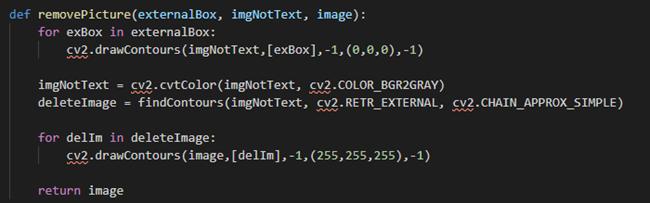
\includegraphics[scale=0.8]{rotate8}
        \caption{ภาพแสดงฟังก์ชั่นการลบรูปภาพออกจากหนังสือ}\label{fig:rotate8}
    \end{figure}

    \begin{figure}[H]
        \centering
        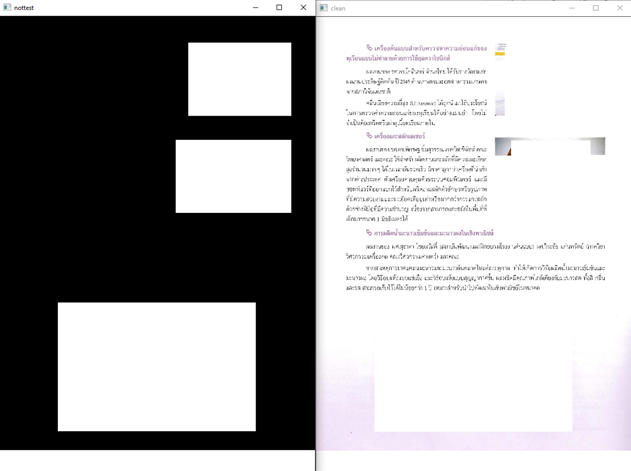
\includegraphics[scale=0.8]{rotate9}
        \caption{ภาพแสดงการสร้าง Mask เพื่อลบรูปภาพ}\label{fig:rotate9}
    \end{figure}

    \begin{figure}[H]
        \centering
        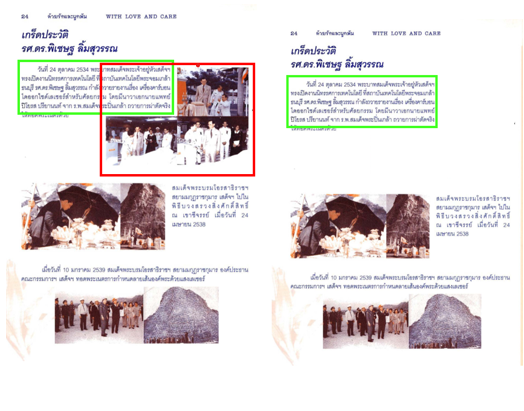
\includegraphics[scale=0.8]{rotate11}
        \caption{ภาพแสดงการสร้าง Mask โดยเว้นที่ตัวหนังสือ}\label{fig:rotate11}
    \end{figure}

    \item การหาค่าเฉลี่ยองศาในแต่ละรูปก็จะนำคอนทัว(contour) ของตัวหนังสือที่ได้มาเข้าสู่กระบวนการวัดมุมและหมุนภาพ โดยการนำจุดสี่จุดของคอนทัว(contour) เล็กมาเฉลี่ย องศาในการหมุน เนื่องจากค่าจุดที่ได้จากการหา minimum area rectangle นั้นอาจจะมีบางครั้งที่ค่าจุดที่ส่งมาไม่ได้เริ่มจากซ้ายบน ดังนั้นจุดและเว้นที่หามาได้นั้นอาจจะทำให้ได้องศาในแนวตั้งมาได้ จึงต้องทำการกรองว่าองศาที่ได้ว่าตั้งฉากหรือไม่ตั้งฉากถ้าเป็นองศาตั้งฉากให้หาการเอียงจากแกน 90 องศา แต่ถ้าไม่ใช่ก็เทียบจากแกนแนวนอน 0 องศาหรือ 180 องศา

    \begin{figure}[H]
        \centering
        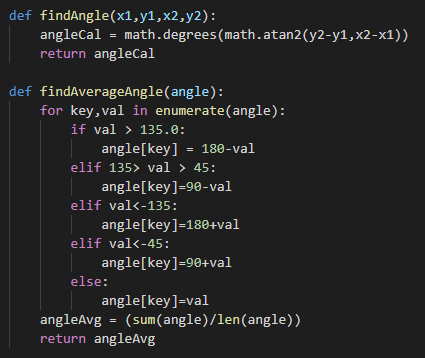
\includegraphics[scale=0.8]{rotate10}
        \caption{ภาพแสดงการหาองศาในการหมุน}\label{fig:rotate10}
    \end{figure}
    
\end{enumerate}

\subsubsection{การลบพื้นหลัง}

จากการที่ฟังก์ชั่นข้ามหน้าได้ผลลัพธ์ที่ไม่ดีพอ จึงเปลี่ยนวิธีการและขั้นตอนการเตรียมข้อมูลรูปภาพใหม่จากความรู้ที่ได้ศึกษาเพิ่มเติมขึ้นมาทำให้นำมาสู่การลบพื้นหลัง

\underline{ขั้นตอนการลบพื้นหลัง}

\begin{enumerate}
    \item แปลงรูปภาพสีให้กลายเป็นขาวดำจะทำให้ชั้นสีเหลือเพียงชั้นเดียวจากเดิมที่มี 3 ชั้นสีเป็น RGB เหลือเป็นค่า Gray scale ที่มีค่า 0-255 โดยที่ค่าเข้าใกล้ 0 คือสีดำและเข้าใกล้ 255 คือสีขาว
    \item นำรูปภาพมาผ่านกระบวนการขยาย(dilate) โดยกำหนดเป็นสี่เหลี่ยมขนาด 5x5 จะได้ผลลัพธ์ดังรูปภาพที่ \ref{fig:rem3}
    \item นำรูปภาพ gray scale มาหารกับค่าที่ถูกขยาย(dilate) มาโดยให้ scale อยู่ที่ 0 – 255 จะทำให้พื้นหลัง หายไปเนื่องจากจะเห็นได้ว่าถ้าส่วนไหนของรูปภาพถูกขยาย(dilate) ออกไปจะไม่ถูกลบเมื่อนำค่าพิกเซลสี(pixel) นั้นมาหารแต่ถ้าพื้นที่นั้นไม่ถูกขยาย(dilate) ออกไปจะทำให้เมื่อนำค่าพิกเซลสี(pixel) มาหารจะทำให้พิกเซลสี(pixel) นั้นกลายเป็นสีขาวดังรูปภาพที่ \ref{fig:rem4}
    \item นำรูปภาพที่ไม่มีพื้นหลัง ไปทำ threshold ให้รูปเหลือเพียงสีขาวกับสีดำ โดยเราจะทำเป็น THRESH\_BINARY\_INV ที่ทำให้ตัวอักษรเป็นสีขาวและพื้นหลังเป็นสีดำเพื่อนำไปใช้ในการหาคอนทัว(contour) ต่อ
    \end{enumerate}

\begin{figure}[H]
    \centering
    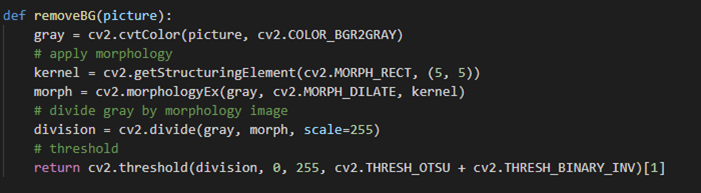
\includegraphics[scale=0.8]{removebg}
    \caption{ภาพแสดงขั้นตอนในการลบพื้นหลังสี}\label{fig:removebg}
\end{figure}

\begin{figure}[H]
    \centering
    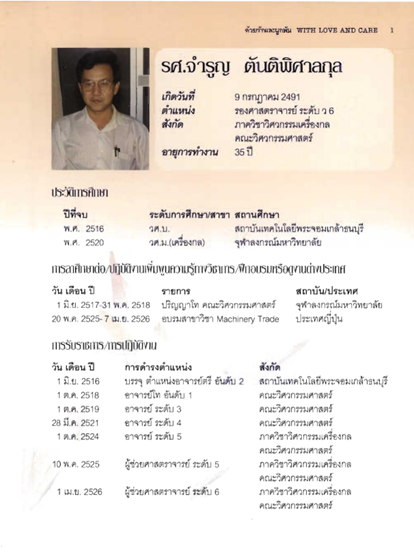
\includegraphics[scale=0.7]{rem1}
    \caption{รูปภาพสีก่อนถูกนำเข้ามาทำการลบพื้นหลัง}\label{fig:rem1}
\end{figure}

\begin{figure}[H]
    \centering
    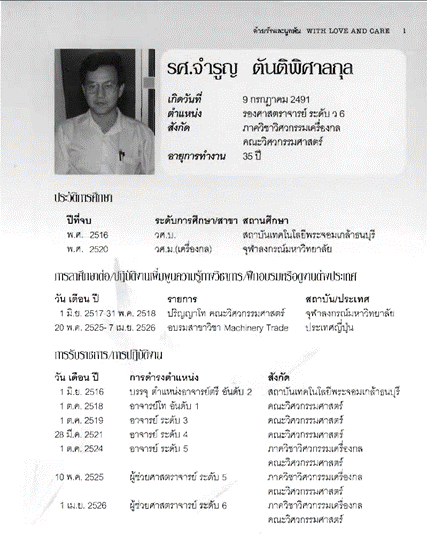
\includegraphics[scale=0.7]{rem2}
    \caption{รูปภาพการแปลงภาพสีเป็น gray scale}\label{fig:rem2}
\end{figure}

\begin{figure}[H]
    \centering
    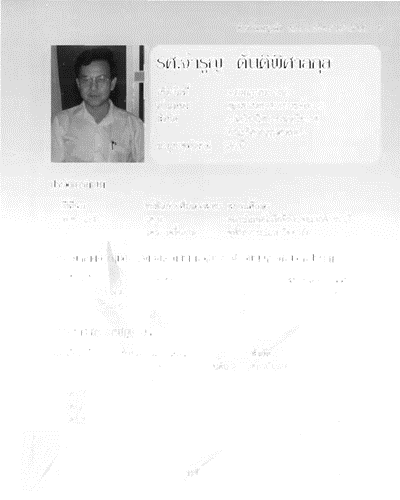
\includegraphics[scale=0.8]{rem3}
    \caption{รูปภาพที่ผ่านการทำการขยาย โดยใช้รูปแบบสี่เหลี่ยมขนาด 5x5}\label{fig:rem3}
\end{figure}

\begin{figure}[H]
    \centering
    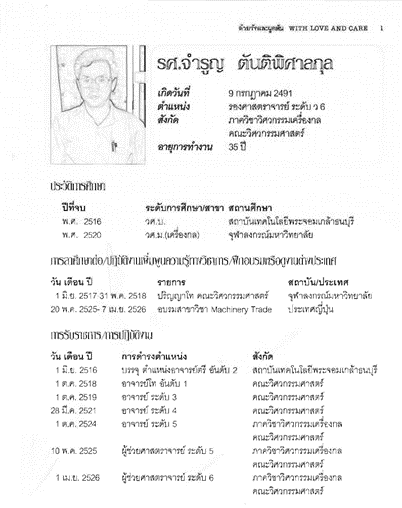
\includegraphics[scale=0.8]{rem4}
    \caption{รูปภาพที่ผ่านการลบพื้นหลัง}\label{fig:rem4}
\end{figure}

\begin{figure}[H]
    \centering
    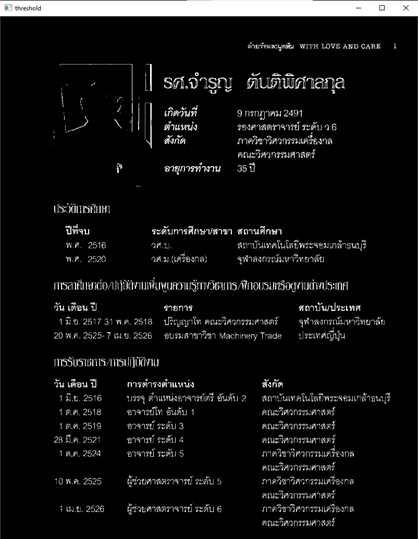
\includegraphics[scale=0.8]{rem5}
    \caption{รูปภาพที่ผ่านทำการ threshold แบบ THRESH\_BINARY\_INV}\label{fig:rem5}
\end{figure}


\subsection{การแปลงข้อมูลรูปภาพให้อยู่ในรูปแบบดิจิทัล}

สำหรับการทำแปลงหนังสือเป็นข้อมูลดิจิตอลจะใช้ Tesseract OCR โดยจะใช้รูปภาพที่ผ่านกระบวนการเตรียมข้อมูลรูปภาพและประโยคที่แปลงออกมาได้จัดเก็บไว้ใช้งานต่อไป

\subsection{การเตรียมข้อมูลตัวหนังสือ}

สำหรับการเตรียมข้อมูลตัวหนังสือ เราจะนำหลักการของการทำ Tokenizer มาใช้ ซึ่งหลักการนี้จะมีรูปแบบแตกต่างกันออกไปในแต่ละภาษาที่จะใช้ โดยภาษาที่เราจะใช้มีภาษาไทย และภาษาอังกฤษ อันดับแรกของกระบวนการทำคือการตัดคำจากรูปประโยคซึ่งระหว่างแต่ละภาษาจะมีรูปแบบต่างกัน เราจึงต้องนำอัลกอรึทึมที่เรียกว่า Deepcut เข้ามาช่วยในการตัดแบ่งคำ หลังจากการตัดคำเราต้องจัดการกับคำที่สื่อความหมายใกล้เคียงกันแต่รูปแบบการเขียนที่แตกต่างกันอย่าง รูปแบบตัวใหญ่ตัวเล็ก คำที่อยู่ในรูปนาม กริยา กรรมแต่สื่อความหมายถึงสิ่งเดียวกัน การจัดการคำที่ไม่มีความหมายแต่เป็นคำสำหรับรูปแบบการพูดเท่านั้น การแก้คำผิดสำหรับคำที่สแกนมาผิดพลาดให้กลายเป็นคำที่ถูกต้อง ซึ่งการเช็คคำในส่วนนี้จะไม่สามารถเช็คคำเฉพาะได้อย่างเช่น ชื่อมหาวิทยาลัย ชื่อคน เราจึงต้องมีการเช็คคำเฉพาะอีกครั้ง และส่วนสุดท้ายผู้ใช้งานจะมีสิทธิในการเช็คคำอีกรอบในขั้นตอนสุดท้ายเพื่อลดการแก้คำผิดที่ไม่สามารถแก้ได้ทั้งหมด

\underline{ขั้นตอนการเตรียมข้อมูลตัวหนังสือ}
\begin{enumerate}
    \item นำแต่ละประโยคในหน้านั้นมาทำการตัดคำโดยใช้อัลกอรึทึม Deepcut
    \item การจัดการตัวอักษรที่เราไม่ต้องการใช้และถือเป็นตัวอักษรที่ผิดพลาดที่เกิดจากการทำ OCR อย่างเช่น รูปแบบตัวอักษาลาติน ตัวอักษรที่เป็นรูปแบบสัญลักษณ์พิเศษ การจัดการรูปตัวอักษาตัวเล็กตัวใหญ่
    \item การค้นหาคำเฉพาะโดยการดูจากบริบทของคำ กรณีภาษาอังกฤษจะเป็นคำที่มีตัวอักษรแรกเป็นตัวใหญ่ และในกรณีของการใช้จุด “.” ของทั้งสองภาษาจะถือว่าเป็นคำเฉพาะเช่นเดียวกัน
    \item นำคำที่ถูกแยกออกมาจากรูปประโยคมาแก้ไขจากคำที่ผิดให้เป็นคำที่ถูกต้อง ซึ่งก่อนแก้ไขต้องระบุว่าคำที่จะแก้ไขเป็นภาษาชนิดใด โดยภาษาไทยจะมีวิธีการตรวจสอบโดยที่คำนั้นจะต้องมีทุกตัวอักษรเป็นภาษาไทยทั้งหมดจึงจะนับว่าเป็นภาษาไทย นอกเหนือจากนั้นจะนับเป็นภาษาอังกฤษทั้งหมด
    \item นำคำที่ถูกแก้คำแล้ว มาแก้คำเฉพาะอีกครั้งนึงเนื่องจากจะมีบางคำที่ไม่สามารถแก้ได้อย่าง ชื่อคนสำคัญ ชื่อมหาวิทยาลัย โดยใช้หลักการ Minimum edit distance
    \item นำผลลัพธ์ที่ได้ส่งไปยังขั้นตอนให้ผู้ใช้ตรวจสอบเพื่อเช็คคำผิดอีกครั้ง
    \item นำผลลัพธ์ที่ผู้ใช้งานตรวจสอบและแก้ไขมาทำการลบคำที่เป็น stop word
    \item นำผลลพธ์ที่ได้จากการทำข้อที่ 7 เข้าสู่ระบบ

\end{enumerate}

\subsection{การสร้างแท็ก}

หลังจากการเตรียมข้อมูลตัวหนังสือ จะนำผลลัพธ์ที่ได้จะนำเข้ากระบวนการสร้างแท็ก โดยอัลกอรึทึม TF-IDF ซึ่งจะถูกเก็บในรูปแบบของ Inverted index ซึ่งในกรณีจากที่กล่าวจะเป็นรูปแบบการสร้างแท็ก ของระบบที่สร้างเอง แต่จะมีในส่วนของการสร้างแท็ก ที่ฝั่งผู้ใช้งานสามารถเพิ่มเข้าไปในระบบเองได้

\underline{ขั้นตอนการสร้างแท็ก}
\begin{enumerate}
    \item นำคำที่ได้จากการเตรียมข้อมูลตัวหนังสือ มาทำการคำนวณผ่านอัลกอรึทึม TF-IDF เพื่อสร้างคะแนนขึ้นมา
    \item นำแท็กผลลัพธ์ที่ได้มาให้ผู้ใช้ตรวจสอบใน 10 อันดับ และสามารถ เพิ่ม ลด แก้ไขได้ โดยที่ระบบจะทำการปรับแก้คะแนนของคำสำคัญที่ผู้ใช้งานจัดการในหนังสือ สามารถถูกค้นหาได้ง่ายกว่าคำสำคัญที่ระบบเป็นสร้างขั้นมาเอง
    
\end{enumerate}

\subsubsection{การอัพเดทค่าคะแนน TF/IDF}

เนื่องจากการที่มีหนังสือเพิ่มเข้ามาในระบบจะทำให้ผลลัพธ์คะแนน TF/IDF เปลี่ยนทั้งระบบจึงทำให้จำเป็นต้องมีการคำนวณใหม่เพื่อความแม่นยำในการค้นหาแต่เนื่องจากถ้าระบบมีหนังสือจำนวนมากยิ่งขึ้นทางผู้จัดทำจึงปรับเปลี่ยนการอัพเดทคะแนนเป็น 1 ครั้งต่อวันโดยที่จะคำนวณคะแนนในช่วงเวลากลางคืนเพื่อไม่ให้ส่งผลกระทบกับผู้ใช้งาน และในส่วนการเพิ่มข้อมูลเข้ามาใหม่คำที่อยู่ภายในหนังสือนั้นจะถูกคำนวณและอัพเดทค่าใหม่ทันทีส่วนคำอื่นนั้นจะต้องรอเวลาที่กำหนดเพื่อที่จะอัพเดทค่า TF IDF และ TF/IDF 

\subsection{การค้นหา}

ในส่วนของระบบการค้นหานั้น จะมีระบบการกรองไว้ให้ผู้ใช้สามารถเลือกได้ว่าจะค้นหาหนังสือในหัวข้อไหน ซึ่งสามารถกรองหัวข้อได้มากกว่า 1 ครั้ง ต่อการค้นหา 1 รอบ โดยระบบการค้นหาจะถูกแบ่งออกเป็นสองส่วน ในส่วนแรกจะเป็นค้นหาในรูปแบบของโคซายซิมิลาริตี้(Cosine Similarity) ซึ่งจะถูกทำ  Tokenizer เพื่อให้การค้นหาของผู้ใช้งานตรงกับฐานข้อมูลมากที่สุด แต่จะไม่ทำการแก้ไขคำเพื่อไม่ให้จุดประสงค์ของการค้นหาถูกเปลี่ยนไปจากเดิม หลังจากนั้นการค้นหาในระบบยังสามารถค้นหาคำใกล้เคียงที่สื่อความหมายแบบเดียวกันจากคำดั้งเดิมเพื่อที่จะได้ผลลัพธ์ที่ครอบคลุมหนังสือมากขึ้น และส่วนที่สองจะเป็นการกรองผลลัพธ์ทำให้ผู้ใช้สามารถลดผลลัพธ์ที่ไม่เกี่ยวข้องจำนวนมากให้ลดน้อยลงเพื่อง่ายต่อการค้นหา เมื่อผู้ใช้งานได้ทำการค้นหาเสร็จสิ้่นระบบจะทำการส่งหนังสือที่เกี่ยวข้องกับมาให้ผู้ใช้งาน

\subsection{การทำโมเดล word2vec}

โดยเราได้เตรียมข้อมูลที่จะนำมาสร้างโมเดลเป็นข้อมูลหนังสือกตเวทิตาและรายงานประจำปีของมหาวิทยาลัยเทคโนโลยีพระจอมเกล้าธนบุรี จำนวนทั้งหมด 43 เล่มโดยจะเป็นการนำข้อมูลที่ถูกกระบวนการ OCR และการเตรียมข้อมูลตัวหนังสือ มาตัดแบ่งคำเว้นช่องว่างและขึ้นบรรทัดใหม่ โดยจะใช้ library genism ในสร้างโมเดลโดยมีการกำหนด window size เท่ากับ 2 และคำต้องมีกล่าวถึงมากกว่า 5 ครั้งโดยทำเป็นลักษณะ CBOW (Continuous Bag of Words)

\underline{ขั้นตอนการเตรียมข้อมูลที่นำมาสร้างโมเดล}

\begin{enumerate}
    \item ทำการแปลงไฟล์หนังสือ PDF ที่ต้องการเป็นไฟล์รูปภาพ
    \item นำรูปภาพผ่านการเตรียมข้อมูลรูปภาพ ในการลบพื้นหลังของรูป
    \item ทำการหาคอนทัว(contour) ในลักษณะสี่เหลี่ยมขนาด 5 x 5 เพื่อเอาไปใช้ในการตัดแบ่งประโยค
    \item ทำการนำประโยคที่ถูกตัดมาทำการ OCR 
    \item นำแต่ละประโยคเข้ากระบวนการเตรียมข้อมูลตัวหนังสือ ในการตัดคำในรูปประโยค
    \item นำคำไปจัดการตัวอักษรที่เราไม่ต้องการใช้และถือเป็นตัวอักษรที่ผิดพลาดที่เกิดจากการทำ OCR
    \item นำคำมาตรวจสอบแก้ไขคำผิดที่เกิดขึ้น
    \item ทำการเว้นช่องว่างระหว่างคำและขึ้นบรรทัดใหม่เมื่อขึ้นประโยคใหม่เพื่อที่เอาไว้ใช้งานสำหรับการสร้างโมเดล
    \item ทำการเขียนเพิ่มลงไปในไฟล์ corpus 
\end{enumerate}

\underline{ขั้นตอนการทำระบบการค้นหา}

\begin{enumerate}
    \item แบ่งแยกประเภทการค้นหาของผู้ใช้ว่ามีค้นหา และการกรองทั้งหมดกี่รูปแบบ
    \item นำรูปประโยค หรือคำ จากรูปแบบการค้นหาที่ได้จากผู้ใช้ไปทำการ ตัดคำผ่าน Deepcut และหาคำที่มีความเหมือนจาก Word2vec
    \item จากผลลัพธ์จะได้คำที่สามารถนำไปหาคะแนนเพื่อเข้ากระบวนการคิดแบบโคซายซิมิลาริตี้(Cosine Similarity) และสามารถได้หนังสือที่เกี่ยวข้องพร้อมอันดับความเกี่ยวข้องของหนังสือนั้น ๆ
    \item จากผลลัพธ์จะได้หนังสือที่เกี่ยวข้อง ดังนั้นหากผู้ใช้ต้องการกรองผลลัพธ์เหล่านี้ระบบจะต้องนำหนังสือไปตรวจสอบว่าหนังสือใดบ้างที่ตรงตามเงื่อนไข
    \item นำผลลัพธ์ที่ได้ส่งคืนให้กลับผู้ใช้งาน

\end{enumerate}

\begin{equation}
    sim(\vec{q},\vec{d})=\frac{\sum_{i=1}^{|v|}q_{i}d_{i} }{\sqrt{\sum_{i=1}^{|v|}q^{2}_{i}x\sqrt{\sum_{i=1}^{|v|}d^{2}_{i}}}}
    \end{equation}    

\subsection{การจัดการหนังสือ}

ในการจัดการข้อมูลหนังสือภายในระบบจะแบ่งทั้ง 3 ส่วนนั้นคือ 1. การเพิ่มหนังสือเข้าสู่ระบบ 2.การแก้ไขหนังสือภายในระบบ  3. การลบหนังสือออกจากระบบ 
ส่วนที่ 1. ในการเพิ่มหนังสือเข้าสู่ระบบ ผู้ใช้งานจะต้องอัปโหลดไฟล์หนังสือในรูปแบบ PDF และกรอกรายละเอียดของหนังสือเพื่อเข้าสู่กระบวนการแปลงหนังสือเป็นรูปภาพต่อไปจะเป็นการเตรียมข้อมูลรูปภาพ ก่อนที่จะนำมาทำการแปลงภาพเป็นตัวอักษรเพื่อที่จะได้ข้อมูลดิจิตอลจากหนังสือที่ผู้ใช้เพิ่มเข้าสู่ระบบหลังจากนั้นจะเป็นการเตรียมข้อมูลตัวหนังสือ และให้ผู้ใช้งานได้ตรวจสอบคำอีกนึงครั้งก่อนที่นำคำเหล่านี้ไปผ่านกระบวนการสร้างแท็ก เพื่อหาคำสำคัญในหนังสือโดยให้ผู้ใช้งานได้ตรวจสอบแก้ไขหรือเพิ่มเติมก่อนจะสิ้นสุดการเพิ่มหนังสือเข้าสู่ระบบ ในส่วนที่ 2 การแก้ไขหนังสือภายในระบบผู้ใช้งานสามารถค้นหาหนังสือภายในระบบเพื่อนำมาแก้ไขรายละเอียดที่ผู้ใช้งานกรอกเท่านั้นแต่มาสามารถแก้ไขคำที่ถูกแปลงออกมาเป็นดิจิตอลอีกครั้งได้ และส่วนสุดท้ายการลบหนังสือในระบบผู้ใช้งานสามารถลบหนังสือภายในระบบได้โดยการค้นหาหนังสือที่ต้องการและกดลบหนังสือนั้นออกจากระบบโดยเมื่อมีการลบหนังสือออกก็จะลบคำที่มีอยู่ในหนังสือออกไปจากระบบเช่นกัน

\subsection{Login}

ผู้ใช้งานสามารถเข้าสู่ระบบเพื่อใช้งานฟังก์ชั่นต่าง ๆภายในระบบโดยเมื่อผู้ใช้งานทำการเข้าสู่ระบบด้วยชื่อผู้ใช้งานและรหัสผ่านแล้วจะได้รับ “token” เพื่อที่จะใช้สำหรับการยืนยันตัวในการใช้ฟังก์ชั่นต่าง ๆภายในระบบและผู้ใช้งานจะสามารถออกจากระบบได้

\section{System requirements}

\underline{ฝั่งผู้ใช้งาน}

ใช้งานได้บนระบบ web browser 

\begin{itemize}
    \item Google Chrome เวอร์ชั่น 84.0 ขึ้นไป 
    \item Microsoft Edge เวอร์ชั่น 83.0 ขึ้นไป
    \item Firefox เวอร์ชั่น 75.0 ขึ้นไป
\end{itemize}
 
\underline{ฝั่งเซิร์ฟเวอร์}
		
ทางด้านฮาร์ดแวร์

        \begin{itemize}
            \item CPU: Intel or AMD processor with 64-bit โดยที่ต้องมี 4 Core ขึ้นไป
            \item GPU: NVIDIA 1050ti or higher
            \item Disk Storage: 10 GB
            \item RAM: 8GB or higher
        \end{itemize}
        
		ทางด้าน Software แบ่งเป็น 2 ส่วนคือ Python และ JavaScript 
        \begin{enumerate}
            \item Python Backend
            \begin{itemize}
                \item Python เวอร์ชั่น 3.7.5
		        \item Tensorflow เวอร์ชั่น 2.3.1
		        \item DeepCut เวอร์ชั่น 0.7
		        \item Django เวอร์ชั่น 3.1.3
		        \item Djangorestframework เวอร์ชั่น 3.12.2
		        \item Django-cors-headers เวอร์ชั่น 3.5.0
		        \item Pythainlp เวอร์ชั่น 2.2.5
		        \item Pyspellchecker เวอร์ชั่น 0.5.5
		        \item nltk เวอร์ชั่น 3.5.0
		        \item mysqlclient เวอร์ชั่น 2.0.1
		        \item pillow เวอร์ชั่น 8.0.1
		        \item shapely เวอร์ชั่น 1.7.1
		        \item pytesseract เวอร์ชั่น 5.0.0 beta
		        \item opencv-python เวอร์ชั่น 4.4.0.46
		        \item pdf2image เวอร์ชั่น 1.14.0
		        \item scipy เวอร์ชั่น 1.5.4
            \end{itemize}
            \item JavaScript Backend and Frontend
		    \begin{itemize}
                \item nodejs เวอร์ชั่น 12.16.3
		        \item apollo-server-express เวอร์ชั่น 2.19.0
		        \item axios เวอร์ชั่น 0.20.0
		        \item cors เวอร์ชั่น 2.8.5
 		        \item dotenv เวอร์ชั่น 8.2.0
		        \item express เวอร์ชั่น 4.17.1
		        \item graphql เวอร์ชั่น 15.4.0
		        \item jsonwebtoken เวอร์ชั่น 8.5.1
		        \item knex เวอร์ชั่น 0.21.5
		        \item morgan เวอร์ชั่น 1.10.0
		        \item mysql2 เวอร์ชั่น 2.2.1
		        \item password-hash เวอร์ชั่น 1.2.2
		        \item react เวอร์ชั่น 16.13.1
		        \item react-hook-form เวอร์ชั่น 6.3.1
		        \item react-router-dom เวอร์ชั่น 5.2.0
		        \item styled-components เวอร์ชั่น 5.1.1
		        \item props-types เวอร์ชั่น 15.7.2
            \end{itemize}
        \end{enumerate}
		
\section{โครงสร้างฐานข้อมูล}

\begin{figure}[H]
    \centering
    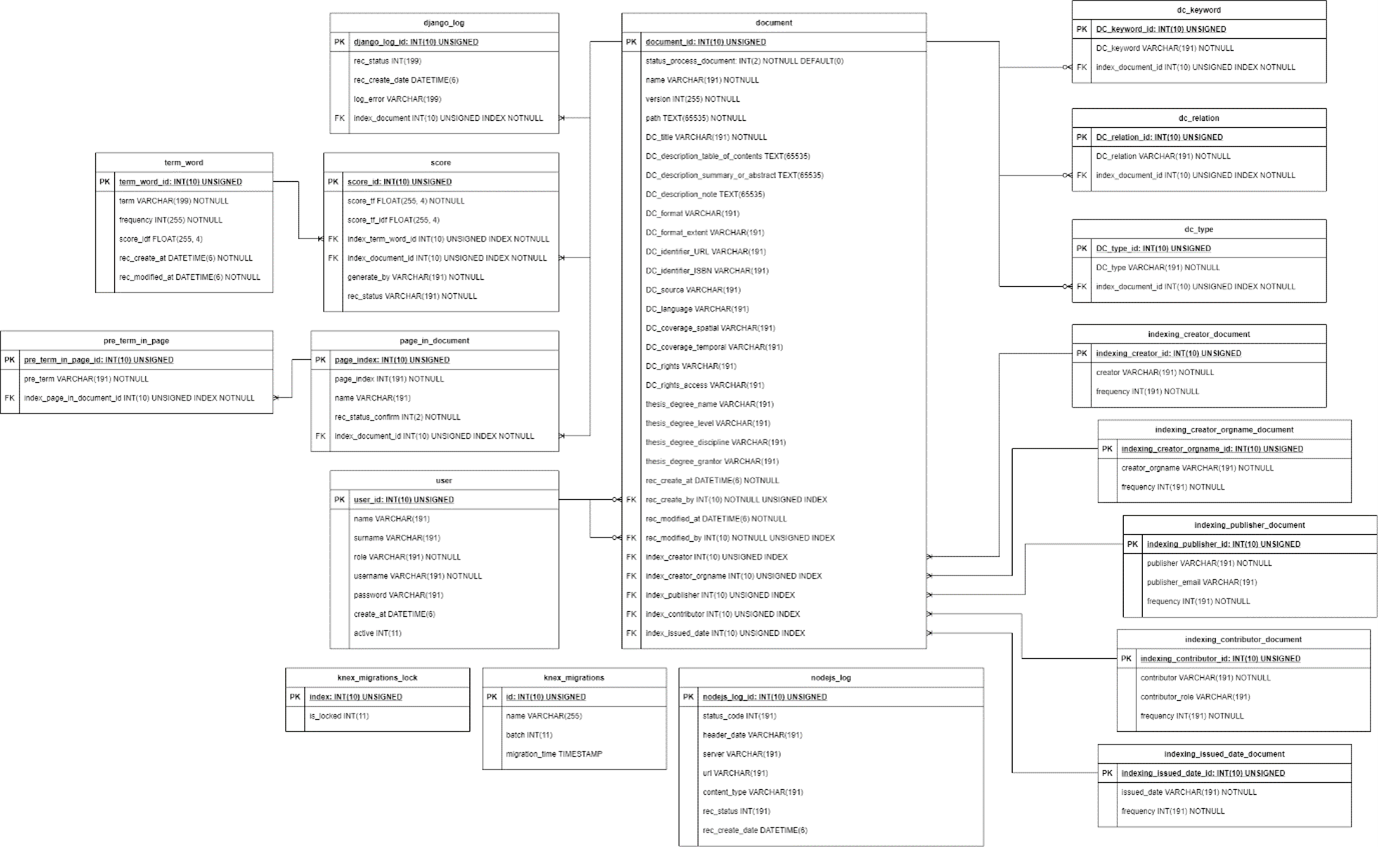
\includegraphics[scale=0.8]{er}
    \caption{แสดง ER Diagram ของฐานข้อมูล}\label{fig:er}
\end{figure}

\begin{figure}[H]
    \centering
    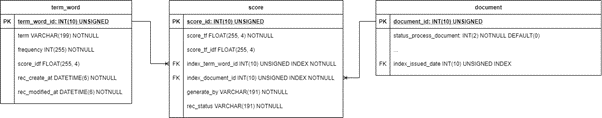
\includegraphics{er1}
    \caption{แสดง ER Diagram ส่วนของคีย์เวิร์ดและคะแนนความสำคัญในระบบ}\label{fig:er1}
\end{figure}


\begin{figure}[H]
    \centering
    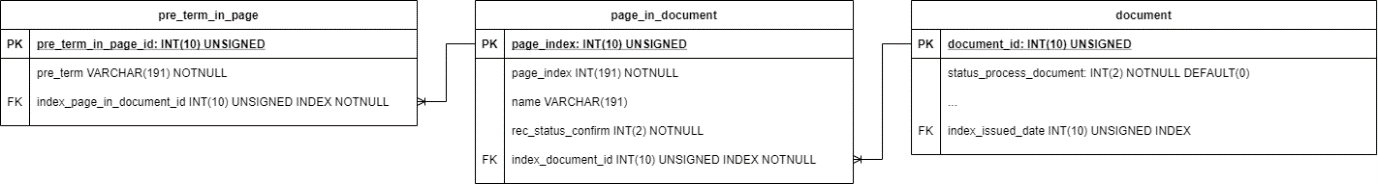
\includegraphics{er2}
    \caption{แสดง ER Diagram ส่วนของการเก็บคำจากแต่ละหน้าที่แปลงมาจากหนังสือ}\label{fig:er2}
\end{figure}


\begin{figure}[H]
    \centering
    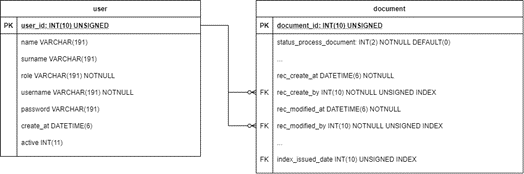
\includegraphics{er3}
    \caption{แสดง ER Diagram ส่วนของประวัติของผู้ใช้งานมีการสร้างหรือแก้ไขหนังสือ}\label{fig:er3}
\end{figure}



\begin{figure}[H]
    \centering
    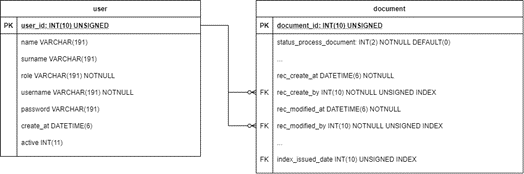
\includegraphics{er4}
    \caption{แสดง ER Diagram ส่วนของการเก็บข้อมูล keyword, relation, type ของหนังสือ}\label{fig:er4}
\end{figure}

\begin{figure}[H]
    \centering
    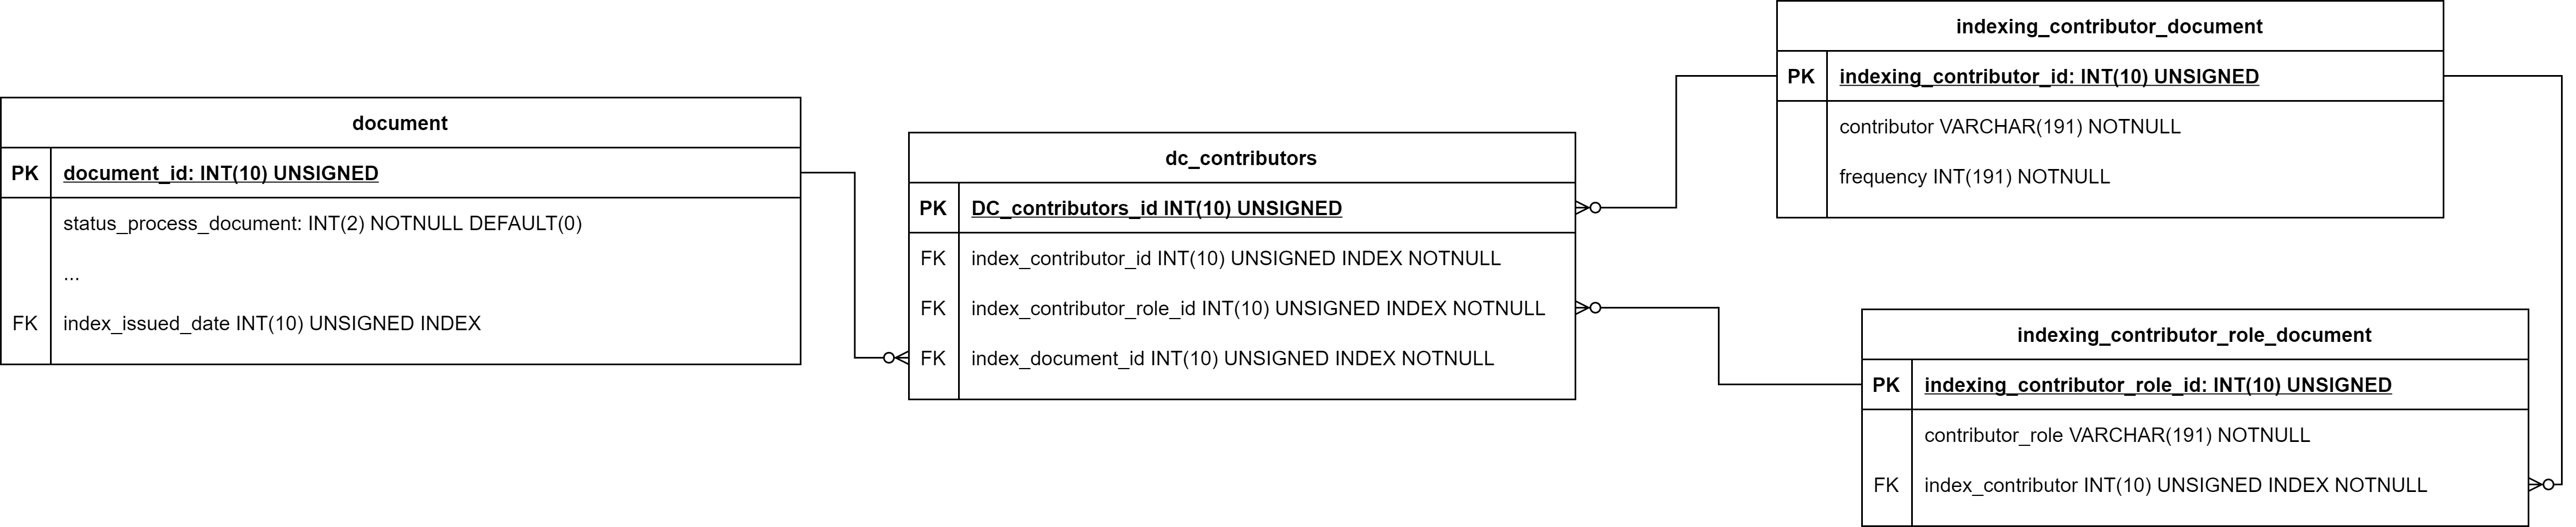
\includegraphics{er5}
    \caption{แสดง ER Diagram ส่วนของการเก็บข้อมูล Contributors ว่ามีความเกี่ยวข้องกับหนังสือไหรบ้าง}\label{fig:er5}
\end{figure}

\begin{figure}[H]
    \centering
    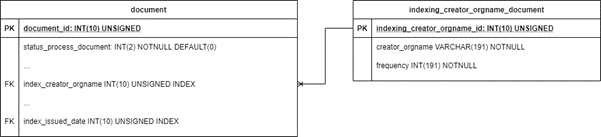
\includegraphics{er6}
    \caption{แสดง ER Diagram ส่วนของ Creator มีความเกี่ยวข้องกับหนังสือไหนบ้าง}\label{fig:er6}
\end{figure}



\begin{figure}[H]
    \centering
    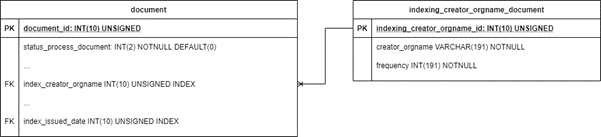
\includegraphics{er7}
    \caption{แสดง ER Diagram ส่วนของ Creator Organized Name มีความเกี่ยวข้องกับหนังสือไหนบ้าง}\label{fig:er7}
\end{figure}



\begin{figure}[H]
    \centering
    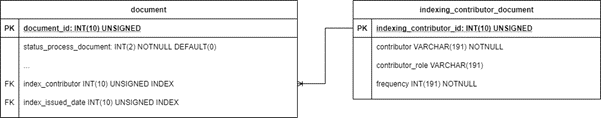
\includegraphics{er8}
    \caption{แสดง ER Diagram ส่วนของ Publisher มีความเกี่ยวข้องกับหนังสือไหนบ้าง}\label{fig:er8}
\end{figure}



\begin{figure}[H]
    \centering
    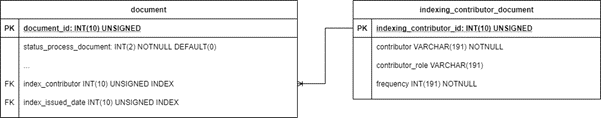
\includegraphics{er9}
    \caption{แสดง ER Diagram ส่วนของ Publisher Email มีความเกี่ยวข้องกับหนังสือไหนบ้าง}\label{fig:er9}
\end{figure}



\begin{figure}[H]
    \centering
    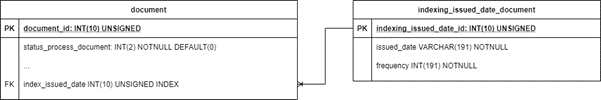
\includegraphics{er10}
    \caption{แสดง ER Diagram ส่วนของ Issued Date มีความเกี่ยวข้องกับหนังสือไหนบ้าง}\label{fig:er10}
\end{figure}



\begin{figure}[H]
    \centering
    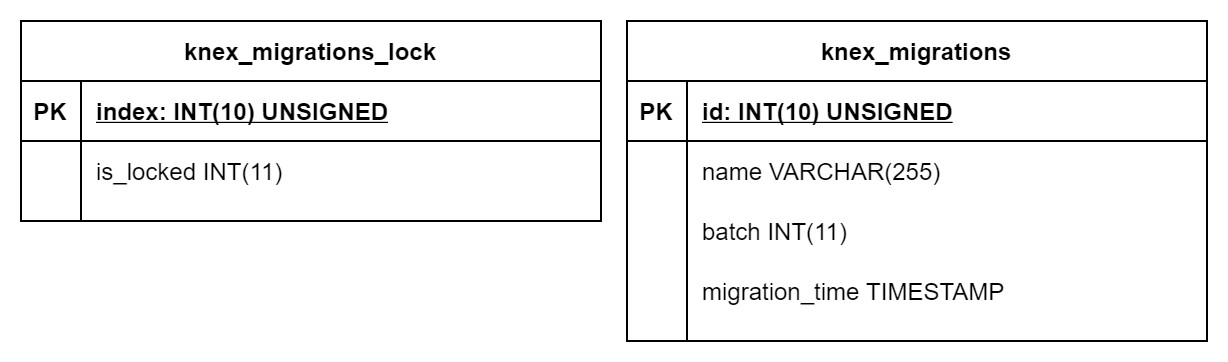
\includegraphics{er11}
    \caption{แสดง ER Diagram ส่วนของ Knex module ที่ใช้สำหรับ Migration ฐานข้อมูล}\label{fig:er11}
\end{figure}



\begin{figure}[H]
    \centering
    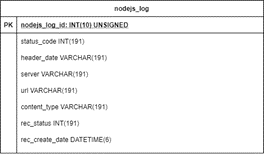
\includegraphics{er12}
    \caption{แสดง ER Diagram ส่วนของการเก็บประวัติการ HTTP Request NodeJS ไปยัง Django}\label{fig:er12}
\end{figure}

\subsection{Database Structure}
รูปที่ \ref{fig:er} แสดงฐานข้อมูลของทั้งระบบโดยจะมีหลัก ๆ ทั้งหมดสามส่วน ทางด้านฝั่งขวาของตาราง document จะเป็นตารางที่เก็บข้อมูลเพิ่มเติมจากตาราง document และส่วนทางด้านฝั่งซ้ายของตาราง document สำหรับการเก็บข้อมูลในด้านของการทำระบบการเก็บคำจากหนังสือที่ถูกใส่ลงมาในระบบ ระบบการแปลงคำเป็นคีย์เวิร์ดและคะแนน TF-IDF ที่นำมาใช้สำหรับการค้นหาหนังสือ ระบบจัดการฐานข้อมูลผู้ใช้งาน และการตรวจสอบความผิดพลาดที่มีโอกาสจากการสร้างคีย์เวิร์ด และส่วนสุดท้ายที่เป็นตารางที่ไม่มีการเชื่อมโยงกับตารางใด ๆ จะมีไว้สำหรับการทำระบบฐานข้อมูล และระบบตรวจสอบ HTTP Request ของทาง NodeJS

รูปที่ \ref{fig:er1} จะเป็นส่วนของคีย์เวิร์ด และคะแนนเพื่อนำมาใช้สำหรับการค้นหาหนังสือของระบบนี้ โดยจะมีทั้งหมดสามตาราง document, term\_word, score ตาราง document จะเป็นตารางที่เก็บข้อมูลของหนังสือไว้ ส่วนตาราง term\_word จะเป็นการเก็บคีย์เวิร์ด และคะแนน IDF สำหรับการลดความสำคัญของคีย์เวิร์ดนั้น ๆ ไว้ซึ่งทั้งสองตารางนี้จะเป็นความสัมพันธ์แบบ one to many กับตาราง score ที่จะมีคะแนนสำหรับระบบการค้นหาเก็บเอาไว้ ที่มีความสัมพันธ์แบบนี้เนื่องจากในแต่ละคีย์เวิร์ดมีโอกาสพบได้ในหลายหนังสือ และหนังสือเองก็สามารถมีได้หลายคีย์เวิร์ด เนื่องจากแต่ละคีย์เวิร์ดที่อยู่ต่างหนังสือกันจะมีคะแนนไม่เท่ากัน

รูปที่ \ref{fig:er2} จะเป็นส่วนของการเก็บคำที่แปลงมาจากหนังสือไว้โดยเริ่มที่ตาราง document จะที่สามารถบอกได้ว่าหนังสือไหน ที่จะมีความพันธ์ one to many ไปยังตาราง page\_in\_document ที่จะเป็นตารางที่บอกถึงหน้าต่าง ๆ ในหนังสือนั้น และยังมีความสัมพันธ์ one to many ต่อไปยังตาราง per\_term\_in\_page ที่จะมีคำต่าง ๆ เก็บเอาไว้ ดังนั้นจะเป็นความสัมพันธ์ที่หนังสือนั้นจะสามารถมีได้หลายหน้า แล้วแต่ละหน้าเองก็จะมีคำต่าง ๆ ที่แปลงออกมาถูกเก็บเอาไว้

รูปที่ \ref{fig:er3} จะเป็นความสัมพันธ์ของบัญชีผู้ใช้กับหนังสือ โดยจะมีตาราง user ที่จะเก็บข้อมูลของผู้ใช้งานที่มีความสัมพันธ์แบบ one to many ไปยังตาราง document ที่จะเก็บต้องเก็บข้อมูลของผู้ใช้ไว้ว่าผู้ใช้คนไหนเป็นคนสร้าง หรือแก้ไขหนังสือนี้ ซึ่งบัญชีผู้ใช้สามารถสร้างหรือแก้ไขหนังสือได้หลายหนังสือ

รูปที่ \ref{fig:er4} จะเป็นส่วนของข้อมูลของตาราง Document เหมือนกันแต่เนื่องจากข้อมูลมีมากกว่าหนึ่งทำให้ต้องสร้างความสัมพันธ์แบบ one to many กับตาราง dc\_keyword, dc\_relation, dc\_type ซึ่งจะเป็นข้อมูลคีย์เวิร์ด ความสัมพันธ์ และประเภทของหนังสือตามลำดับ

รูปที่ \ref{fig:er5} จะเป็นการเก็บข้อมูลของ Contributor โดยจะมีตารางแยกเพื่อเก็บของสัมพันธ์ของทั้งสองด้านเนื่องจากในหนังสือสามารถมี contributor ได้หลายคน และ contributor สามารถมีหลายหนังสือเช่นกัน โดยที่ contributor จะมี role เป็นของตัวเองซึ่งสามารถมีหลาย role เช่นกันทำให้ต้องมีตาราง รองรับเพิ่ม

รูปที่ \ref{fig:er6} จะเป็นส่วนของการเก็บความสัมพันธ์ระหว่าง Creator กับหนังสือ เนื่องจาก Creator สามารถมีได้หลายหนังสือทำให้ตาราง indexing\_creator\_document จะเป็นความสัมพันธ์แบบ one to many กับตาราง document 

รูปที่ \ref{fig:er7} จะเป็นส่วนของการเก็บความสัมพันธ์ระหว่าง Creator orgname กับหนังสือเนื่อง จากCreator orgname สามารถมีได้หลายหนังสือทำให้ตาราง indexing\_creator\_orgname\_document จะเป็นความสัมพันธ์แบบ one to many กับตาราง document 

รูปที่ \ref{fig:er8} จะเป็นส่วนของการเก็บความสัมพันธ์ระหว่าง Publisher กับหนังสือ เนื่องจาก Publisher สามารถมีได้หลายหนังสือทำให้ตาราง indexing\_publisher\_document จะเป็นความสัมพันธ์แบบ one to many กับตาราง document 

รปที่ \ref{fig:er9} จะเป็นส่วนของการเก็บความสัมพันธ์ระหว่าง Publisher Email กับหนังสือ เนื่องจาก Publisher Email สามารถมีได้หลายหนังสือทำให้ตาราง indexing\_publisher\_email\_document จะเป็นความสัมพันธ์แบบ one to many กับตาราง document

รูปที่ \ref{fig:er10} จะเป็นส่วนของการเก็บความสัมพันธ์ระหว่าง Issued Date กับหนังสือ เนื่องจาก Issued Date สามารถมีได้หลายหนังสือทำให้ตาราง indexing\_issued\_date\_document จะเป็นความสัมพันธ์แบบ one to many กับตาราง document 

รูปที่ \ref{fig:er11} จะเป็นสองตารางที่บันทึกการจัดการฐานข้อมูลของเครื่องมือที่ชื่อว่า Knex ที่จะทำการจัดการสร้างฐานข้อมูล ด้วยคำสั่ง Migration แล้วหลังจากทำคำสั่งเสร็จสิ้นจะเก็บบันทึกไว้

รูปที่ \ref{fig:er12} จะเป็นตารางสำหรับการเก็บ HTTP Request จาก NodeJS ที่ส่งไปทางฝั่งของ Django ซึ่งจะถูกเก็บข้อมูลไว้ในตารางนี้

\subsection{Database Dictionary}

อธิบายถึงชื่อของคอลัมน์ ความหมายและลักษณะการเก็บข้อมูลภายในฐานข้อมูลโดยที่ตารางมีทั้งหมด 18 ตารางดังนี้



\begin{table}[H]
\caption{ตารางอธิบายความหมายตาราง term\_word}\label{tbl:termword}
\begin{tabular}{|l|l|l|}
\hline
\multicolumn{3}{|c|}{term\_word}                                                                                                                            \\ \hline
\multicolumn{1}{|c|}{ชื่อคอลัมน์} & \multicolumn{1}{c|}{ความหมาย}            & \multicolumn{1}{c|}{ประเภท}                                                  \\ \hline
term\_word\_id                    & id สำหรับบ่งบอกคำศัพท์                   & \begin{tabular}[c]{@{}l@{}}INT (10) PK \\ Auto\_Increment\end{tabular}       \\ \hline
term                              & คำศัพท์                                  & VARCHAR (191)                                                                \\ \hline
frequency                         & จำนวนความถี่ของหนังสือที่มีคำศัพท์นี้อยู่ & INT (191)                                                                    \\ \hline
score\_idf                        & คะแนน idf ของคำศัพท์นี้                  & FLOAT (255,4)                                                                \\ \hline
rec\_create\_at                   & วันเวลาของการเพิ่มคำศัพท์นี้เข้าสู่ระบบ  & \begin{tabular}[c]{@{}l@{}}DATETIME (6) \\ current\_timestamp\end{tabular}   \\ \hline
rec\_modified\_at                 & วันเวลาที่อัปเดทข้อมูลของคำศัพท์         & \begin{tabular}[c]{@{}l@{}}DATETIME   (6) \\ current\_timestamp\end{tabular} \\ \hline
\end{tabular}
\end{table}

\begin{table}[H]
\caption{ตารางอธิบายความหมายตาราง user}\label{tbl:user}
\begin{tabular}{|l|l|l|}
\hline
\multicolumn{3}{|c|}{user}                                                                                                                                   \\ \hline
\multicolumn{1}{|c|}{ชื่อคอลัมน์} & \multicolumn{1}{c|}{ความหมาย}             & \multicolumn{1}{c|}{ประเภท}                                                  \\ \hline
user\_id                          & id สำหรับบ่งบอกผู้ใช้งาน                  & \begin{tabular}[c]{@{}l@{}}INT   (10) PK \\ Auto\_Increment\end{tabular}     \\ \hline
name                              & ชื่อของผู้ใช้งาน                          & VARCHAR (50)                                                                 \\ \hline
surname                           & นามสกุลของผู้ใช้งาน                       & VARCHAR (191)                                                                \\ \hline
role                              & ตำแหน่งของผู้ใช้งาน                       & VARCHAR (191)                                                                \\ \hline
username                          & ชื่อผู้ใช้งานสำหรับทำการ login            & VARCHAR (191)                                                                \\ \hline
password                          & รหัสผ่านผู้ใช้งานสำหรับทำการ login        & VARCHAR (191)                                                                \\ \hline
create\_at                        & วันเวลาของผู้ใช้งานของการเพิ่มเข้าสู่ระบบ & \begin{tabular}[c]{@{}l@{}}DATETIME   (6) \\ current\_timestamp\end{tabular} \\ \hline
active                            & สถานะการระงับบัญชีผู้ใช้งาน               & \begin{tabular}[c]{@{}l@{}}INT   (11) \\ Default 1\end{tabular}              \\ \hline
\end{tabular}
\end{table}

\begin{table}[H]
\caption{ตารางอธิบายความหมายตาราง score}\label{tbl:score}        
\begin{tabular}{|l|l|l|}
\hline
\multicolumn{3}{|c|}{score}                                                                                                                       \\ \hline
\multicolumn{1}{|c|}{ชื่อคอลัมน์} & \multicolumn{1}{c|}{ความหมาย}  & \multicolumn{1}{c|}{ประเภท}                                                  \\ \hline
score\_id                         & id สำหรับบ่งบอกคะแนนของคำศัพท์ & \begin{tabular}[c]{@{}l@{}}INT (10) PK \\ Auto\_Increment\end{tabular}       \\ \hline
score\_tf                         & คะแนน tf ของคำศัพท์            & FLOAT (255,4)                                                                \\ \hline
score\_tf\_idf                    & คะแนน tf-idf ของคำศัพท์        & FLOAT   (255,4)                                                              \\ \hline
index\_term\_word\_id             & id สำหรับบ่งบอกคำศัพท์         & INT   (10)                                                                   \\ \hline
index\_document\_id               & id สำหรับบ่งบอกหนังสือ          & INT   (10)                                                                   \\ \hline
generate\_by                      & คะแนนถูกคำนวณโดยใคร            & \begin{tabular}[c]{@{}l@{}}VARCHAR   (191) \\ Default ‘default’\end{tabular} \\ \hline
rec\_status                       & สถานะการใช้คะแนนนี้            & \begin{tabular}[c]{@{}l@{}}INT   (191) \\ Default 1\end{tabular}             \\ \hline
\end{tabular}
\end{table}

\begin{table}[H]
\caption{ตารางอธิบายความหมายตาราง pre\_term\_in\_page}\label{tbl:preterminpage}        
\begin{tabular}{|l|l|l|}
\hline
\multicolumn{1}{|c|}{ชื่อคอลัมน์} & \multicolumn{1}{c|}{ความหมาย}                                      & \multicolumn{1}{c|}{ประเภท}                                                   \\ \hline
pre\_term\_in\_page\_id           & id   สำหรับบ่งบอกคำศัพท์ชั่วคราวที่รอให้ผู้ใช้งานตรวจสอบ           & \makecell[l]{INT   (10) PK\\Auto\_Increment} \\ \hline
pre\_term                         & คำศัพท์ชั่วคราวที่รอให้ผู้ใช้ตรวจสอบ                               & VARCHAR   (191)                                                               \\ \hline
index\_page\_in\_document\_id     & id   สำหรับบ่งบอกที่อยู่ของคำศัพท์ชั่วคราวที่รอให้ผู้ใช้งานตรวจสอบ & INT (10) FK                                                                   \\ \hline
\end{tabular}
\end{table}

\begin{table}[H]
\caption{ตารางอธิบายความหมายตาราง page\_in\_document}\label{tbl:pageindocument}        
\begin{tabular}{|l|l|l|}
\hline
\multicolumn{3}{|c|}{page\_in\_document}                                                                                             \\ \hline
\multicolumn{1}{|c|}{ชื่อคอลัมน์} & \multicolumn{1}{c|}{ความหมาย}                                    & \multicolumn{1}{c|}{ประเภท}   \\ \hline
page\_in\_document\_id            & id สำหรับบ่งบอกที่อยู่ของคำศัพท์ชั่วคราวที่รอให้ผู้ใช้งานตรวจสอบ & \begin{tabular}[c]{@{}l@{}}INT (10) PK\\ Auto\_Increment\end{tabular} \\ \hline
page\_index                       & หน้าของหนังสือ                                                    & INT (191)                     \\ \hline
name                              & ชื่อ File ของข้อมูล                                              & VARCHAR (191)                 \\ \hline
rec\_status\_confirm              & สถานะการยืนยันโดยผู้ใช้งาน                                       & \begin{tabular}[c]{@{}l@{}}INT (2) PK\\ Default 2\end{tabular}            \\ \hline
index\_document\_id               & id สำหรับบ่งบอกหนังสือ                                            & INT (10) FK                   \\ \hline
\end{tabular}
\end{table}

\begin{table}[H]
\caption{ตารางอธิบายความหมายตาราง nodejs\_log}\label{tbl:nodejslog}        
\begin{tabular}{|l|l|l|}
\hline
\multicolumn{3}{|c|}{nodejs\_log}                                                                                                                                  \\ \hline
\multicolumn{1}{|c|}{ชื่อคอลัมน์} & \multicolumn{1}{c|}{ความหมาย}                   & \multicolumn{1}{c|}{ประเภท}                                                  \\ \hline
nodejs\_log\_id                   & id สำหรับการจัดเก็บประวัติการทำงานฝั่ง nodejs   & \begin{tabular}[c]{@{}l@{}}INT   (10) PK \\ Auto\_Increment\end{tabular}     \\ \hline
status\_code                      & เก็บสถานะ HTTP หลังจากที่ส่งไปแล้วว่าได้สถานะใด & INT (191)                                                                    \\ \hline
header\_date                      & เก็บข้อมูล header ของ HTTP ที่ส่งไป             & VARCHAR (191)                                                                \\ \hline
server                            & ชื่อรูปแบบของเซิฟเวอร์ที่ส่งไป                  & VARCHAR (191)                                                                \\ \hline
url                               & ตำแหน่งโดเมนหรือ IP ที่ส่งไป                    & INT (10) FK                                                                  \\ \hline
content\_type                     & รูปแบบเนื้อหาที่ส่งไป                           & VARCHAR (191)                                                                \\ \hline
rec\_status                       & สถานะที่บอกว่าการส่งเกิดข้อผิดพลาดระหว่างทาง    & INT (191)                                                                    \\ \hline
rec\_create\_date                 & วันเวลาที่ทำการส่ง   ณ ตอนนั้น                  & \begin{tabular}[c]{@{}l@{}}DATETIME   (6) \\ current\_timestamp\end{tabular} \\ \hline
\end{tabular}
\end{table}

\begin{table}[H]
\caption{ตารางอธิบายความหมายตาราง knex\_migrations\_lock}\label{tbl:knexmigrationslock}        
\begin{tabular}{|l|l|l|}
\hline
\multicolumn{3}{|c|}{knex\_migrations\_lock}                                                                                                          \\ \hline
\multicolumn{1}{|c|}{ชื่อคอลัมน์} & \multicolumn{1}{c|}{ความหมาย}            & \multicolumn{1}{c|}{ประเภท}                                            \\ \hline
index                             & id บ่งบอกลำดับของไฟล์ migration ของ knex & \begin{tabular}[c]{@{}l@{}}INT (10) PK \\ Auto\_Increment\end{tabular} \\ \hline
is\_locked                        & สถานะของไฟล์ migration                   & INT (11)                                                               \\ \hline
\end{tabular}
\end{table}

\begin{table}[H]
\caption{ตารางอธิบายความหมายตาราง knex\_migrations}\label{tbl:knexmigrations}        
\begin{tabular}{|l|l|l|}
\hline
\multicolumn{3}{|c|}{knex\_migrations}                                                                                                                        \\ \hline
\multicolumn{1}{|c|}{ชื่อคอลัมน์} & \multicolumn{1}{c|}{ความหมาย}                    & \multicolumn{1}{c|}{ประเภท}                                            \\ \hline
id                                & id บ่งบอกลำดับการทำงานของไฟล์ migration ของ knex & \begin{tabular}[c]{@{}l@{}}INT (10) PK \\ Auto\_Increment\end{tabular} \\ \hline
name                              & ชื่อไฟล์ migration ที่ถูกทำงานเรียบร้อย          & VARCHAR (255)                                                          \\ \hline
batch                             & ลำดับที่                                         & INT (11)                                                               \\ \hline
migration\_time                   & เวลาที่ถุกสั่งให้ทำงาน                           & \begin{tabular}[c]{@{}l@{}}TIMESTAMP\\ current\_timestamp\end{tabular} \\ \hline
\end{tabular}
\end{table}

\begin{table}[H]
\caption{ตารางอธิบายความหมายตาราง indexing\_publisher\_document}\label{tbl:indexingpublisherdocument}        
\begin{tabular}{|l|l|l|}
\hline
\multicolumn{3}{|c|}{indexing\_publisher\_document}                                                                                             \\ \hline
\multicolumn{1}{|c|}{ชื่อคอลัมน์} & \multicolumn{1}{c|}{ความหมาย}      & \multicolumn{1}{c|}{ประเภท}                                            \\ \hline
indexing\_publisher\_id           & id สำหรับบ่งบอกสำนักพิมพ์          & \begin{tabular}[c]{@{}l@{}}INT (10) PK \\ Auto\_Increment\end{tabular} \\ \hline
publisher                         & ชื่อสำนักพิมพ์                     & VARCHAR (191)                                                          \\ \hline
frequency                         & จำนวนของสำนักพิมพ์นี้ที่ถูกอ้างอิง & INT (191)                                                              \\ \hline
\end{tabular}
\end{table}


\begin{table}[H]
\caption{ตารางอธิบายความหมายตาราง indexing\_publisher\_email\_document}\label{tbl:indexingpublisherdocument}            
\begin{tabular}{|l|l|l|}
\hline
\multicolumn{3}{|c|}{indexing\_publisher\_email\_document}                                                                                      \\ \hline
\multicolumn{1}{|c|}{ชื่อคอลัมน์} & \multicolumn{1}{c|}{ความหมาย}      & \multicolumn{1}{c|}{ประเภท}                                            \\ \hline
indexing\_publisher\_email\_id    & id สำหรับบ่งบอกสำนักพิมพ์          & \begin{tabular}[c]{@{}l@{}}INT (10) PK \\ Auto\_Increment\end{tabular} \\ \hline
publisher\_email                  & e-mail ของสำนักพิมพ์               & VARCHAR (191)                                                          \\ \hline
frequency                         & จำนวนของสำนักพิมพ์นี้ที่ถูกอ้างอิง & INT (191)                                                              \\ \hline
\end{tabular}
\end{table}

\begin{table}[H]
\caption{ตารางอธิบายความหมายตาราง indexing\_issued\_date\_document}\label{tbl:indexingissueddatedocument}        
\begin{tabular}{|l|l|l|}
\hline
\multicolumn{3}{|c|}{indexing\_issued\_date\_document}                                                                                                 \\ \hline
\multicolumn{1}{|c|}{ชื่อคอลัมน์} & \multicolumn{1}{c|}{ความหมาย}             & \multicolumn{1}{c|}{ประเภท}                                            \\ \hline
indexing\_issued\_date\_id        & id สำหรับบ่งบอกปีที่เขียน                 & \begin{tabular}[c]{@{}l@{}}INT (10) PK \\ Auto\_Increment\end{tabular} \\ \hline
issued\_date                      & วันเวลาของปีที่เขียนหนังสือ                & DATE                                                                   \\ \hline
frequency                         & จำนวนของวันเวลาของปีที่เขียนที่ถูกอ้างอิง & INT (191)                                                              \\ \hline
\end{tabular}
\end{table}

\begin{table}[H]
\caption{ตารางอธิบายความหมายตาราง indexing\_creator\_orgname\_document}\label{tbl:indexingcreatororgnamedocument}        
\begin{tabular}{|l|l|l|}
\hline
\multicolumn{3}{|c|}{indexing\_creator\_orgname\_document}                                                                                                \\ \hline
\multicolumn{1}{|c|}{ชื่อคอลัมน์} & \multicolumn{1}{c|}{ความหมาย}                & \multicolumn{1}{c|}{ประเภท}                                            \\ \hline
indexing\_creator\_orgname\_id    & id สำหรับบ่งบอกชื่อหน่วยงานรับผิดชอบสังกัด   & \begin{tabular}[c]{@{}l@{}}INT (10) PK \\ Auto\_Increment\end{tabular} \\ \hline
creator\_orgname                  & ชื่อหน่วยงานรับผิดชอบสังกัด                  & VARCHAR (191)                                                          \\ \hline
frequency                         & จำนวนของหน่วยงานรับผิดชอบสังกัดที่ถูกอ้างอิง & INT (191)                                                              \\ \hline
\end{tabular}
\end{table}

\begin{table}[H]
\caption{ตารางอธิบายความหมายตาราง indexing\_creator\_document}\label{tbl:indexingcreatordocument}
\begin{tabular}{|l|l|l|}
\hline
\multicolumn{3}{|c|}{indexing\_creator\_document}                                                                                                \\ \hline
\multicolumn{1}{|c|}{ชื่อคอลัมน์} & \multicolumn{1}{c|}{ความหมาย}       & \multicolumn{1}{c|}{ประเภท}                                            \\ \hline
indexing\_creator\_id             & id สำหรับบ่งบอกชื่อผู้เขียนหนังสือ   & \begin{tabular}[c]{@{}l@{}}INT (10) PK \\ Auto\_Increment\end{tabular} \\ \hline
creator                           & ชื่อของผู้เขียนหนังสือ               & VARCHAR (191)                                                          \\ \hline
frequency                         & จำนวนของผู้เขียนหนังสือที่ถูกอ้างอิง & INT (191)                                                              \\ \hline
\end{tabular}
\end{table}


\begin{table}[H]
\caption{ตารางอธิบายความหมายตาราง dc\_contributors}\label{tbl:dccontributor}
\begin{tabular}{|l|l|l|}
\hline
\multicolumn{3}{|c|}{dc\_contributors}                                                                                                      \\ \hline
\multicolumn{1}{|c|}{ชื่อคอลัมน์} & \multicolumn{1}{c|}{ความหมาย}                                             & \multicolumn{1}{c|}{ประเภท} \\ \hline
dc\_contributors\_id              & id สำหรับบ่งบอกข้อมูลความสัมพันธ์ของชื่อหน่วยข้อมูลผู้ร่วมงาน   กับหนังสือ & \begin{tabular}[c]{@{}l@{}}INT (10) PK\\ Auto\_Increment\end{tabular} \\ \hline
index\_contributor\_id            & id สำหรับบ่งบอกชื่อผู้เขียนหนังสือ                                         & INT(10) FK                  \\ \hline
index\_document\_id               & id สำหรับบ่งบอกชื่อหน่วยข้อมูลผู้ร่วมงาน                                  & INT(10) FK                  \\ \hline
\end{tabular}
\end{table}

\begin{table}[H]
\caption{ตารางอธิบายความหมายตาราง indexing\_contributor\_document}\label{tbl:indexingcontributordocument}
\begin{tabular}{|l|l|l|}
\hline
\multicolumn{3}{|c|}{indexing\_contributor\_document}                                                        \\ \hline
\multicolumn{1}{|c|}{ชื่อคอลัมน์} & \multicolumn{1}{c|}{ความหมาย}              & \multicolumn{1}{c|}{ประเภท} \\ \hline
indexing\_contributor\_id         & id   สำหรับบ่งบอกชื่อหน่วยข้อมูลผู้ร่วมงาน & \begin{tabular}[c]{@{}l@{}}INT (10) PK\\ Auto\_Increment\end{tabular}   \\ \hline
contributor                       & ชื่อหน่วยข้อมูลผู้ร่วมงาน                  & VARCHAR (191)               \\ \hline
frequency                         & จำนวนของหน่วยข้อมูลผู้ร่วมงานที่ถูกอ้างอิง & INT (191)                   \\ \hline
\end{tabular}
\end{table}

\begin{table}[H]
\caption{ตารางอธิบายความหมายตาราง indexing\_contributor\_role\_document}\label{tbl:indexingcontributorroledocument}
\begin{tabular}{|l|l|l|}
\hline
\multicolumn{3}{|c|}{indexing\_contributor\_role\_document}                                                                                        \\ \hline
\multicolumn{1}{|c|}{ชื่อคอลัมน์} & \multicolumn{1}{c|}{ความหมาย}              & \multicolumn{1}{c|}{ประเภท}                                       \\ \hline
indexing\_contributor\_role\_id   & id   สำหรับบ่งบอกตำแหน่งของผู้ร่วมงาน      & \begin{tabular}[c]{@{}l@{}}INT(10)\\ Auto\_Increment\end{tabular} \\ \hline
contributor\_role                 & ชื่อตำแหน่งของผู้ร่วมงาน                   & VARCHAR (191)                                                     \\ \hline
index\_contributor                & id   สำหรับบ่งบอกชื่อหน่วยข้อมูลผู้ร่วมงาน & INT (191)                                                         \\ \hline
\end{tabular}
\end{table}


\begin{table}[H]
\caption{ตารางอธิบายความหมายตาราง dc\_type}\label{tbl:dctype}
\begin{tabular}{|l|l|l|}
\hline
\multicolumn{3}{|c|}{dc\_type}                                                                                                               \\ \hline
\multicolumn{1}{|c|}{ชื่อคอลัมน์} & \multicolumn{1}{c|}{ความหมาย}   & \multicolumn{1}{c|}{ประเภท}                                              \\ \hline
DC\_type\_id                    & id สำหรับบ่งบอกประเภทของหนังสือ & \begin{tabular}[c]{@{}l@{}}INT (10) PK  \\ Auto\_Increment\end{tabular} \\ \hline
DC\_type                        & ประเภทของหนังสือ                & VARCHAR   (191)                                                         \\ \hline
index\_document\_id             & id สำหรับบ่งบอกหนังสือ          & INT   (10)                                                             \\ \hline
\end{tabular}
\end{table}

\begin{table}[H]
\caption{ตารางอธิบายความหมายตาราง dc\_relation}\label{tbl:dcrelation}
\begin{tabular}{|l|l|l|}
\hline
\multicolumn{3}{|c|}{dc\_relation}                                                                      \\ \hline
\multicolumn{1}{|c|}{ชื่อคอลัมน์} & \multicolumn{1}{c|}{ความหมาย}        & \multicolumn{1}{c|}{ประเภท}  \\ \hline
DC\_relation\_id                  & id   สำหรับบ่งบอกหนังสือที่เกี่ยวข้อง & \begin{tabular}[c]{@{}l@{}}INT (10) PK\\ Auto\_Increment\end{tabular} \\ \hline
DC\_relation                      & ชื่อหนังสือที่เกี่ยวข้อง              & VARCHAR   (191)              \\ \hline
index\_document\_id               & id สำหรับบ่งบอกหนังสือ                & INT   (10)                   \\ \hline
\end{tabular}
\end{table}

\begin{table}[H]
\caption{ตารางอธิบายความหมายตาราง dc\_keyword}\label{tbl:dckeyword}
\begin{tabular}{|l|l|l|}
\hline
\multicolumn{3}{|c|}{dc\_keyword}                                                                \\ \hline
\multicolumn{1}{|c|}{ชื่อคอลัมน์} & \multicolumn{1}{c|}{ความหมาย} & \multicolumn{1}{c|}{ประเภท}  \\ \hline
DC\_keyword\_id                   & id   สำหรับบ่งบอกคำสัญ         & \begin{tabular}[c]{@{}l@{}}INT (10) PK\\ Auto\_Increment\end{tabular} \\ \hline
DC\_keyword                       & คำศัพท์                       & VARCHAR   (191)              \\ \hline
index\_document\_id               & id สำหรับบ่งบอกหนังสือ         & INT   (10)                   \\ \hline
\end{tabular}
\end{table}

% \begin{table}[H]
% \caption{ตารางอธิบายความหมายตาราง document}\label{tbl:document}
% \vspace*{-1.25em}
% \end{table}
\begin{longtable}[l]{|l|l|l|}
\caption{ตารางอธิบายความหมายตาราง document}
\label{tbl:document}
\endfirsthead
\endhead

\hline
\multicolumn{1}{|c|}{ชื่อคอลัมน์}      & \multicolumn{1}{c|}{ความหมาย}                    & \multicolumn{1}{c|}{ประเภท}                                                       \\ \hline 
document\_id                         & id สำหรับบ่งบอกหนังสือ                                        & \begin{tabular}[c]{@{}l@{}}INT(10)   \\ Auto\_Increment\end{tabular} \\ \hline
status\_process\_document            & สถานะการทำงานของหนังสือ                                       & INT   (2)                                                            \\ \hline
name                                 & ชื่อไฟล์ PDF หนังสือ                                          & VARCHAR   (191)                                                      \\ \hline
version                              & ครั้งที่ตีพิมพ์                                              & INT   (191)                                                          \\ \hline
page\_start                          & หน้าหนังสือที่กำหนดเป็นหน้าเริ่ม                              & INT   (191)                                                          \\ \hline
amount\_page                         & จำนวนหน้าทั้งหมดของหนังสือ                                    & INT   (191)                                                          \\ \hline
path                                 & ตำแหน่งไฟล์ PDF ที่ผู้ใช้งานอัปโหลดเข้าสู่ระบบ               & TEXT                                                                 \\ \hline
path\_image                          & ตำแหน่งไฟล์รูปภาพของหนังสือ                                   & TEXT                                                                 \\ \hline
name                                 & ชื่อไฟล์ PDF หนังสือ                                          & VARCHAR (191)                                                        \\ \hline
DC\_title                            & ชื่อหนังสือ                                                   & VARCHAR (191)                                                        \\ \hline
DC\_title\_alternative               & ชื่อรองของหนังสือ                                             & VARCHAR (191)                                                        \\ \hline
DC\_description\_table\_of\_contents & สาระสำคัญที่มาจากสารบัญ                                      & TEXT                                                                 \\ \hline
DC\_description\_note                & รายละเอียดทั่วไปของหนังสือ                                    & TEXT                                                                 \\ \hline
DC\_description\_summary             & สาระสำคัญของข้อมูลสารสนเทศที่ผ่านการค้นหา   รวบรวม วิเคราะห์ & TEXT                                                                 \\ \hline
DC\_description\_abstract            & ข้อมูลสรุปจากบทคัดย่อ   วิทยานิพนธ์ และเนื้อหา               & TEXT                                                                 \\ \hline
DC\_format                           & รูปแบบข้อมูลที่ถูกจัดเก็บในระบบ                              & VARCHAR (191)                                                        \\ \hline
DC\_format\_extent                   & ขนาดของไฟล์หนังสือ                                            & VARCHAR (191)                                                        \\ \hline
DC\_identifier\_URL                  & แหล่งที่มาของหนังสือ                                          & VARCHAR   (191)                                                      \\ \hline
DC\_identifier\_ISBN                 & เลขมาตราฐานสากลของหนังสือ                                     & VARCHAR   (191)                                                      \\ \hline
DC\_source                           & หน่วยข้อมูลต้นฉบับ                                           & VARCHAR   (191)                                                      \\ \hline
DC\_language                         & ภาษาของหนังสือ                                                & VARCHAR   (191)                                                      \\ \hline
DC\_coverage\_spatial                & สถานที่ของหนังสือที่เป็นเจ้าของ                               & VARCHAR   (191)                                                      \\ \hline
DC\_coverage\_temporal               & ช่วงเวลาในหน่วยปีของหนังสือ                                   & VARCHAR   (191)                                                      \\ \hline
DC\_rights                           & ระดับการเข้าถึงของข้อมูล                                     & VARCHAR   (191)                                                      \\ \hline
DC\_rights\_access                   & ตำแหน่งที่มีสิทธิ์ในการเข้าถึงข้อมูล                         & VARCHAR   (191)                                                      \\ \hline
thesis\_degree\_name                 & ชื่อเต็มของปริญญา                                            & VARCHAR   (191)                                                      \\ \hline
thesis\_degree\_level                & ระดับของปริญญา                                               & VARCHAR   (191)                                                      \\ \hline
thesis\_degree\_discipline           & สาขาวิชา                                                     & VARCHAR   (191)                                                      \\ \hline
thesis\_degree\_grantor              & มหาวิทยาลัย                                                  & VARCHAR   (191)                                                      \\ \hline
index\_creator                       & id สำหรับบ่งบอกชื่อผู้เขียนหนังสือ                            & INT   (10) FK                                                        \\ \hline
index\_creator\_orgname              & id สำหรับบ่งบอกชื่อหน่วยงานรับผิดชอบสังกัด                   & INT   (10) FK                                                        \\ \hline
index\_publisher                     & id สำหรับบ่งบอกสำนักพิมพ์                                    & INT   (10) FK                                                        \\ \hline
index\_publisher\_email              & id สำหรับบ่งบอกอีเมล์สำนักพิมพ์                              & INT   (10) FK                                                        \\ \hline
index\_issued\_date                  & id สำหรับบ่งบอกปีที่เขียน                                    & INT   (10) FK                                                        \\ \hline
rec\_create\_at                      & วันเวลาของหนังสือที่ถูกนำเข้าสู่ระบบ         & \begin{tabular}[c]{@{}l@{}}DATETIME   (6)   \\ current\_timestamp \end{tabular}             \\ \hline
rec\_create\_by                      & id สำหรับบ่งบอกผู้ใช้งานที่นำหนังสือเข้าสู่ระบบ               & INT   (10) FK                                                        \\ \hline
rec\_modified\_at                    & วันเวลาของหนังสือที่ถูกแก้ไขข้อมูล           & \begin{tabular}[c]{@{}l@{}}DATETIME   (6)   \\ current\_timestamp \end{tabular}            \\ \hline
rec\_modified\_by                    & id สำหรับบ่งบอกผู้ใช้งานที่แก้ไขหนังสือในระบบ                 & INT   (10) FK                                                        \\ \hline
rec\_status                          & ค่าสถานะของหนังสือสำหรับการใช้งาน                            & INT   (2)                                                            \\ \hline
\end{longtable}

\section{UML Design}
\subsection{Use case diagram}

\begin{figure}[H]
    \centering
    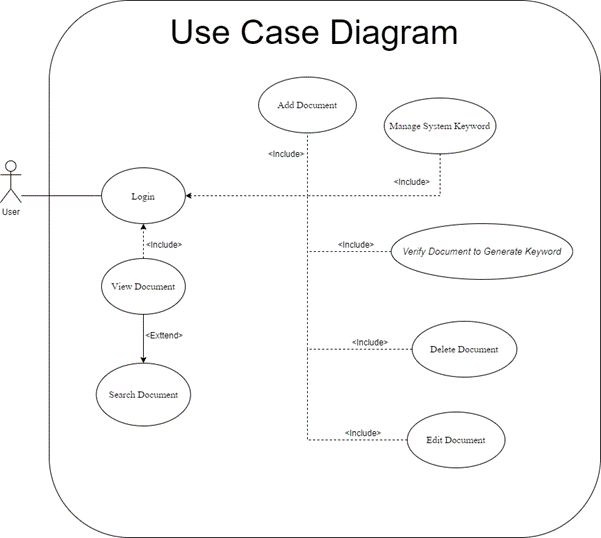
\includegraphics{usecasediagram}
    \caption{Use case diagram}\label{fig:usecasediagram}
\end{figure}

\subsection{Sequence diagram}

\subsubsection{Use case Add Document}

Scenario 1: เพิ่มหนังสือ/หนังสือเข้าสู่ระบบ

Goal: เพิ่มข้อมูลของหนังสือเข้าไปอยู่ในระบบ

Precondition: กดไปที่หัวข้อ INSERT BOOK ใน Web Application 

Main success scenario:

\begin{enumerate}
    \item อัพโหลดหนังสือ/หนังสือเลือกหน้าที่จะให้เริ่มต้นการแปลง
    \item กรอกข้อมูลรายละเอียดที่ต้องการลงในระบบ
    \item แสดงสถานะของการเพิ่มข้อมูล
    \item เพิ่มหนังสือ/หนังสือเข้าสู่ระบบ
\end{enumerate}

\begin{figure}[H]
    \centering
    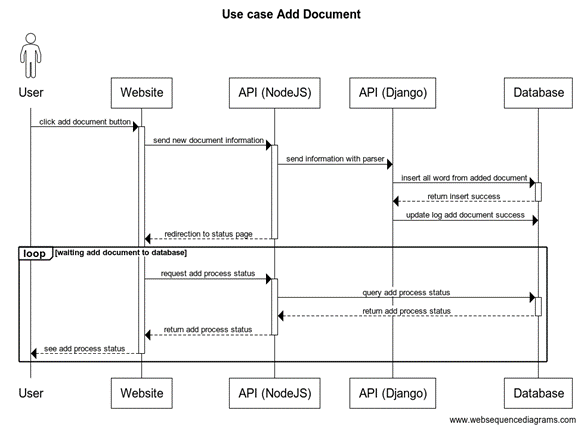
\includegraphics{scene1}
    \caption{แสดง Scenario 1 เพิ่มหนังสือเข้าระบบ}\label{fig:scene1}
\end{figure}

\subsubsection{Use case Manage word in document}

Scenario 2: การตรวจสอบและแก้ไขคำก่อนนำเข้าสู่ระบบ

Goal: ผู้ใช้งานเห็นคำที่จะถูกการแปลงเป็นดิจิตอลแล้วสามารถจัดการคำเหล่านั้นได้

Precondition: อยู่ภายในขั้นตอนการเพิ่มหนังสือ/หนังสือลงในระบบ

Main success scenario:

\begin{enumerate}
    \item ผู้ใช้เข้าไปยังหน้าดูสถานะการเพิ่มหนังสือ
    \item ผู้ใช้เลือกหนังสือที่อยู่ในสถานะตรวจสอบคำ
    \item ระบบแสดงคำทั้งหมดที่ถูกแปลงมาได้จากหนังสือแต่ละหน้า
    \item ผู้ใช้ตรวจสอบ แก้ไขคำที่แสดงขึ้นมา
    \item ยืนยันขั้นตอนการตรวจสอบและแก้ไขคำ
\end{enumerate}
\begin{figure}[H]
    \centering
    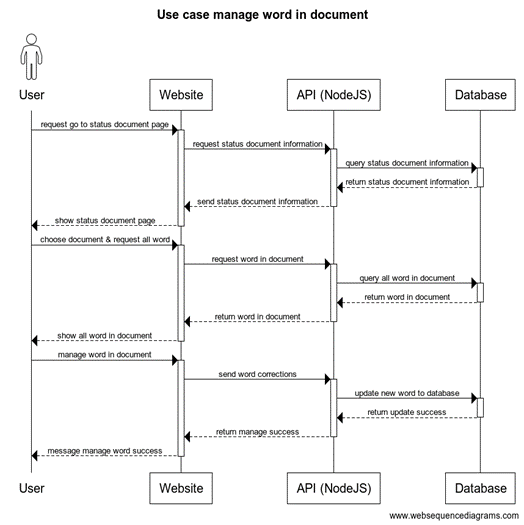
\includegraphics{scene2}
    \caption{แสดง Scenario 2 การจัดการคำที่ถูกเก็บได้จากหนังสือในระบบ}\label{fig:scene2}
\end{figure}

\subsubsection{Use case Verify Document to Generate Keyword}

Scenario 3: ยื่นหนังสือว่าพร้อมสำหรับการถูกนำไปสร้างคียเวิร์ด

Goal: หนังสือถูกยืนยันพร้อมกับสร้างคีย์เวิร์ดเพื่อเพิ่มเข้าไปในระบบ

Precondition: ไปยังหน้าสถานะของหนังสือแล้วกดไปยังปุ่มยืนยันหนังสือถูกต้อง

Main success scenario:

\begin{enumerate}
    \item ผู้ใช้เข้าไปยังหน้าดูสถานะการเพิ่มหนังสือ
    \item ระบบแสดงสถานะหนังสือว่าหนังสือไหนอยู่สถานะใดแล้วบ้าง
    \item ผู้ใช้กดยืนยันว่าหนังสือถูกต้อง
    \item ระบบย้ายไปหน้าสถานะหนังสืออีกครั้งเพื่อรอผลการทำงาน
    \item ระบบแสดงการยืนยันหนังสือ และถูกเพื่อคีย์เวิร์ดเสร็จสิ้น
\end{enumerate}
\begin{figure}[H]
    \centering
    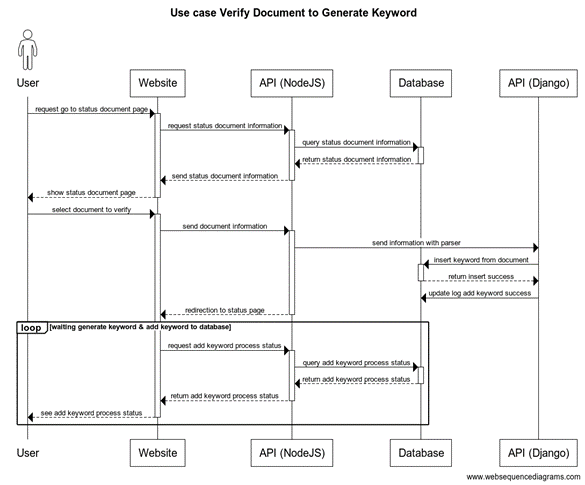
\includegraphics{scene3}
    \caption{แสดง Scenario 3 ยืนหนังสือว่าพร้อมสำหรับการถูกนำไปสร้างคีย์เวิร์ด}\label{fig:scene3}
\end{figure}

\subsubsection{Use case Edit Document}

Scenario 4: การแก้ไขรายละเอียดของหนังสือ/หนังสือที่อยู่ภายในระบบ

Goal: รายละเอียดหนังสือถูกแก้ไขตามผู้ใช้งานต้องการ

Precondition: กดไปที่หัวข้อ MANAGE BOOK ใน Web Application

Main success scenario:

\begin{enumerate}
    \item ผู้ใช้ค้นหาหนังสือที่ต้องการแก้ไขรายละเอียด
    \item แสดงผลลัพธ์ในการค้นหาหนังสือ/หนังสือ
    \item เลือกหนังสือ/หนังสือที่ต้องการแก้ไขรายละเอียด
    \item แก้ไขรายละเอียดที่ต้องการ
    \item กดบันทึกข้อมูลลงไปในระบบ
\end{enumerate}
\begin{figure}[H]
    \centering
    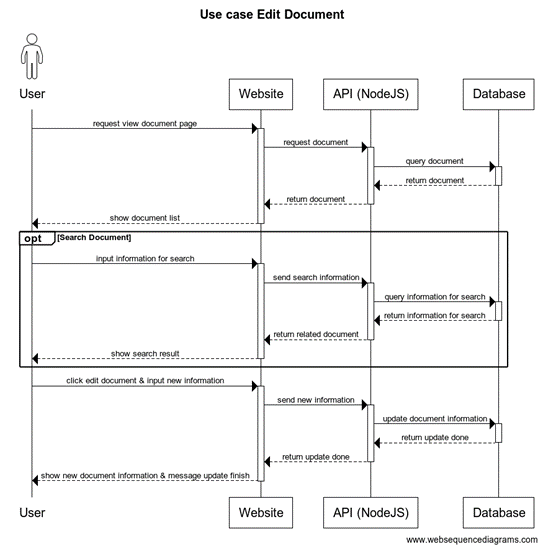
\includegraphics{scene4}
    \caption{แสดง Scenario 4 แก้ไขข้อมูลหนังสือ}\label{fig:scene4}
\end{figure}

\subsubsection{Use case Delete Document}

Scenario 5: ลบหนังสือ/หนังสือภายในระบบ

Goal: หนังสือ/หนังสือถูกนำออกจากระบบ

Precondition: กดเลือกหัวข้อ MANAGE BOOK ใน Web Application

Main success scenario:

\begin{enumerate}
    \item ผู้ใช้ทำการค้นหาหนังสือหนังสือที่ต้องการจะลบออกจากระบบ
    \item แสดงผลลัพธ์ในการค้นหาหนังสือ/หนังสือ
    \item กดลบหนังสือ/หนังสือที่ต้องการ
    \item กดยืนยันคำสั่งลบเพื่อบันทึกลงระบบ
\end{enumerate}
\begin{figure}[H]
    \centering
    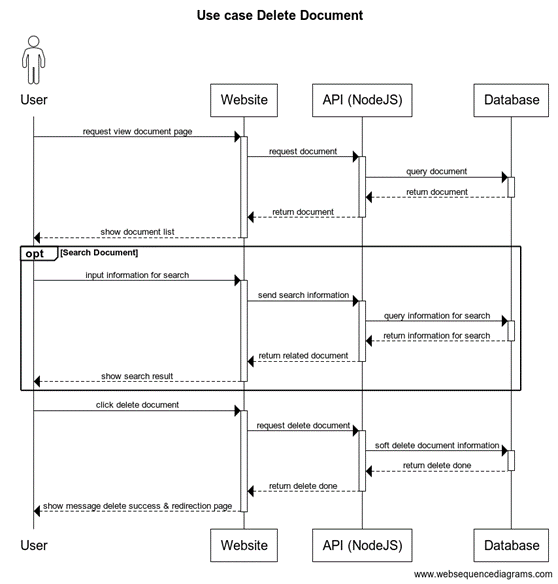
\includegraphics{scene5}
    \caption{แสดง Scenario 5 ลบหนังสือ}\label{fig:scene5}
\end{figure}

\subsubsection{Use case View Document \& Search Document}

Scenario 6: ดูข้อมูลหนังสือ และการค้นหาหนังสือ

Goal: ผู้ใช้เจอหนังสือที่ต้องการ

Precondition: กดไปที่หัวข้อ SEARCH ใน Web Application

Main success scenario:

\begin{enumerate}
    \item กรอกรายละเอียดข้อมูลที่ต้องการจะค้นหา
    \item แสดงผลลัพธ์ในการค้นหา
    \item ผู้ใช้เลือกหนังสือที่ต้องการที่จะดูข้อมูล
    \item ระบบย้ายไปยังหน้าแสดงข้อมูลหนังสือที่ถูกเลือก
\end{enumerate}
\begin{figure}[H]
    \centering
    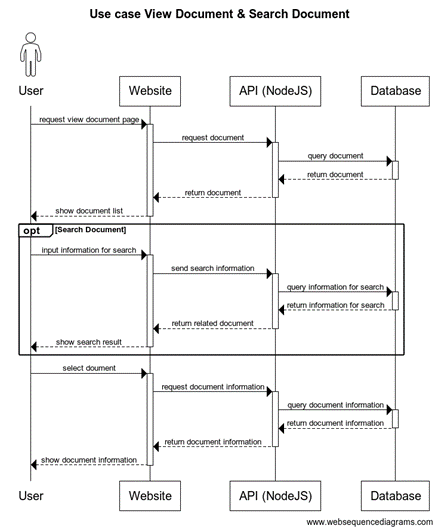
\includegraphics{scene6}
    \caption{แสดง Scenario 6 ดูข้อมูลหนังสือ และการค้นหาหนังสือ}\label{fig:scene6}
\end{figure}

\subsubsection{Use case Login}

Scenario 7: ระบบล็อกอิน

Goal: เพื่อเข้าสู่ระบบให้สามารถใช้ฟังก์ชั่นภายใน Web Application เพิ่มเติมได้

Precondition: กดหัวข้อ LOGIN ใน Web Application

Main success scenario:

\begin{enumerate}
    \item ผู้ใช้กรอกชื่อผู้ใช้งานและรหัสผ่าน
    \item กดเข้าสู่ระบบ
    \item เข้าสู่ระบบสำเร็จ ส่งผู้ใช้กลับไปสู่ Homepage
    \item สามารถเข้าใช้งานฟังก์ชั่นของ Web Application ได้
\end{enumerate}
\begin{figure}[H]
    \centering
    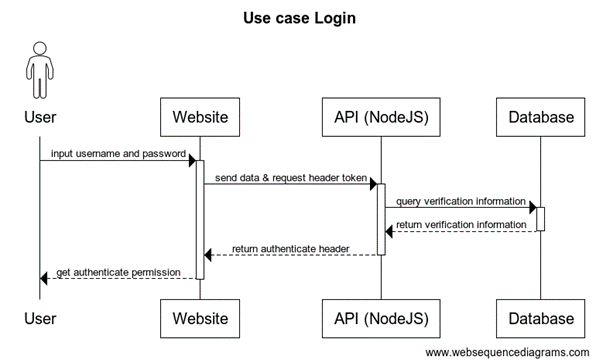
\includegraphics{scene7}
    \caption{แสดง Scenario 7 ระบบล็อกอิน}\label{fig:scene7}
\end{figure}

\section{GUI Design}

\subsection{Homepage}
\begin{figure}[H]
    \centering
    
\includegraphics[scale=0.3]{hp}
    \caption{ภาพแสดงหน้าหลักของเว็บไซต์}\label{fig:hp}
\end{figure}
หน้าหลักของเว็บไซต์จะเป็นหน้าที่เน้นการค้นหาเป็นหลัก ที่ผู้ใช้สามารถเข้าถึงเมนูการเพิ่มหนังสือ การจัดการ และการเข้าสู่ระบบได้ที่แถบ Navigation ด้านบนของเว็บไซต์ดังรูปที่ \ref{fig:hp}

\subsection{Homepage2}
\begin{figure}[H]
    \centering
    
\includegraphics[scale=0.3]{hp2}
    \caption{ภาพแสดงหน้าหลักของเว็บไซต์หลังจากการกดเปิดเมนู}\label{fig:hp2}
\end{figure}
เมื่อกดปุ่มลูกศรที่ด้านล่างของรูป \ref{fig:hp} จะมีเมนูเพิ่มเติมขึ้นมากลายเป็นรูปที่ \ref{fig:hp2} ซึ่งจะแสดงรายละเอียดในแต่ละฟังก์ชั่นเพิ่มเติม

\subsection{Login}
\begin{figure}[H]
    \centering
    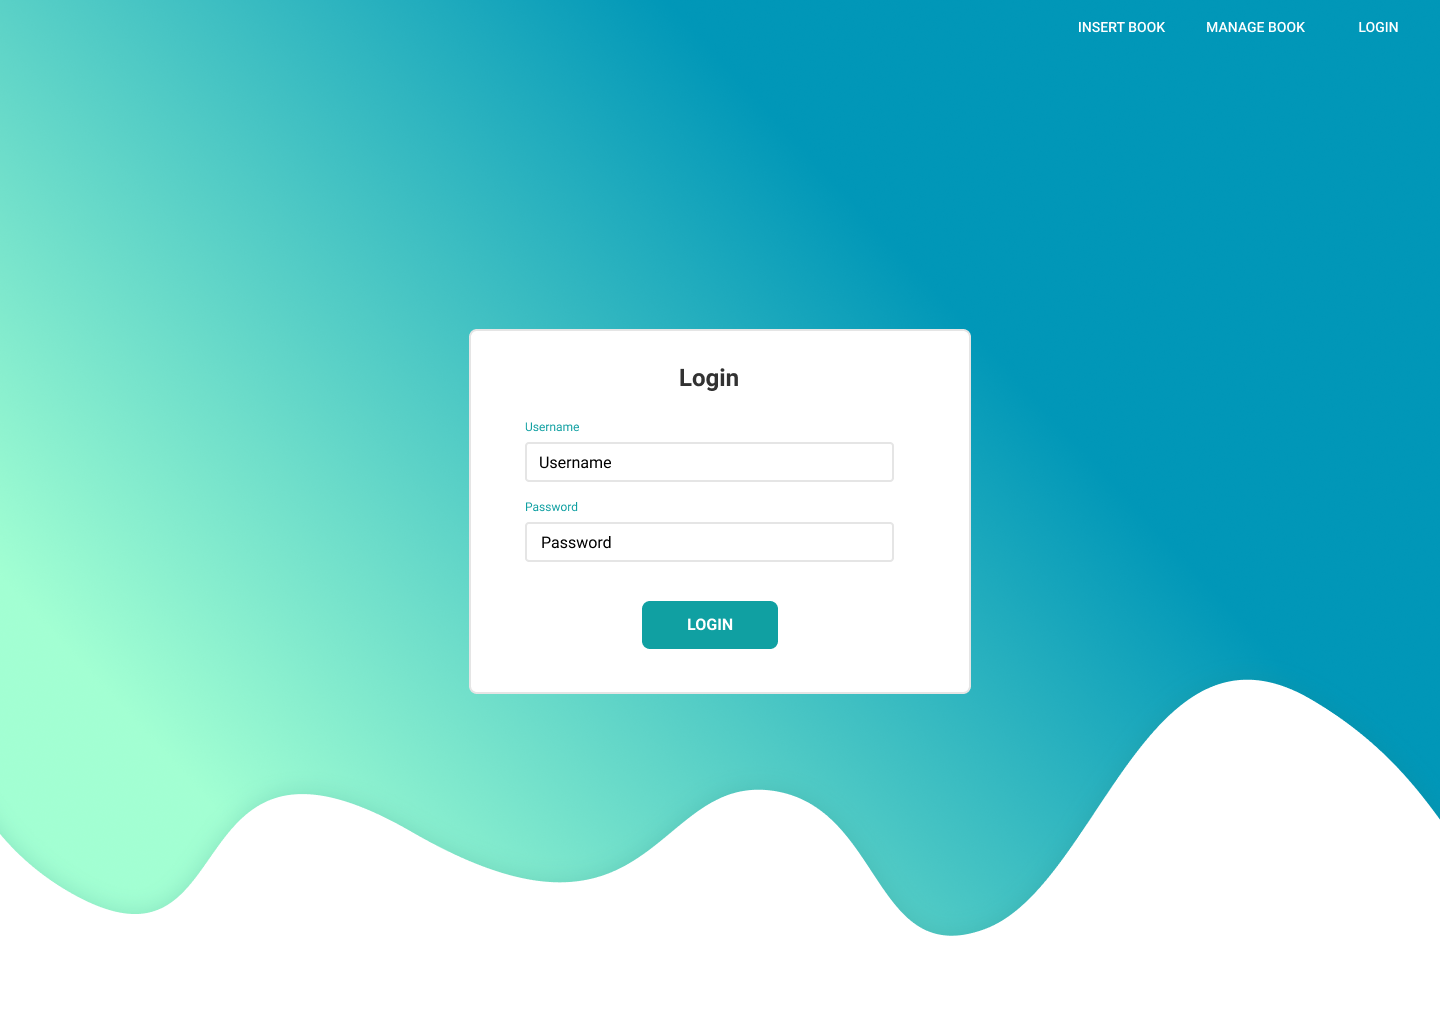
\includegraphics[scale=0.3]{login}
    \caption{ภาพแสดงหน้าเข้าสู่ระบบ}\label{fig:scene7}
\end{figure}
ก่อนที่จะทำการเพิ่มหนังสือหรือจัดการกับหนังสือผู้ใช้นั้นจะต้องเข้าสู่ระบบก่อนเสมอ ถ้าเกิดกดเข้าฟังก์ชั่นการเพิ่มหนังสือหรือค้นหาโดยที่ยังไม่ได้เข้าสู่ระบบ ระบบจะบังคับให้ผู้ใช้เข้ามาในหน้าเข้าสู่ระบบดังรูป 3.25 เพื่อทำการเข้าสู่ระบบหรือจะเข้ามาโดยการกด log in ที่ปุ่มขวาบนได้

\subsection{Insert Book(1)}
\begin{figure}[H]
    \centering
    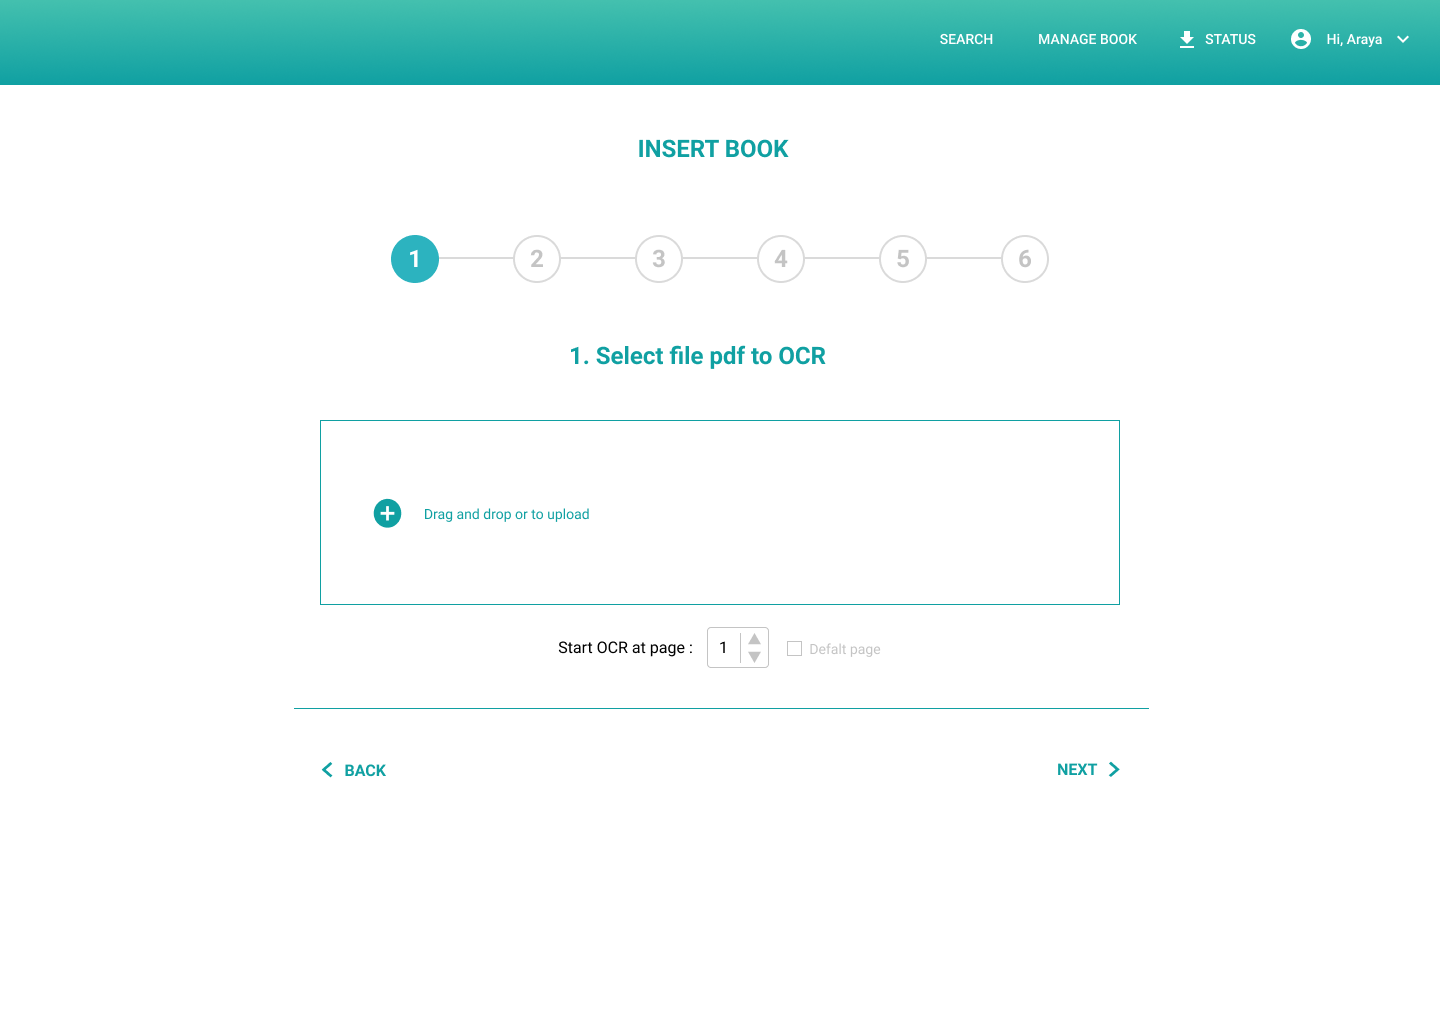
\includegraphics[scale=0.27]{i1}
    \caption{ภาพแสดงขั้นตอนการเพิ่มหนังสือเข้าสู่ระบบขั้นเลือกไฟล์}\label{fig:i1}
\end{figure}
หน้าเพิ่มหนังสือขั้นแรกจะเป็นการเลือกไฟล์หนังสือที่ต้องการโดยที่จะมีส่วนของการเพิ่มไฟล์ที่อยู่รูปของ pdf เพื่อทำ OCR จากนั้นจะสามารถเลือกได้ว่าจะทำการ OCR ตั้งแต่หน้าไหนดังรูปที่ 3.26

\subsection{Insert Book (2) }
\begin{figure}[H]
    \centering
    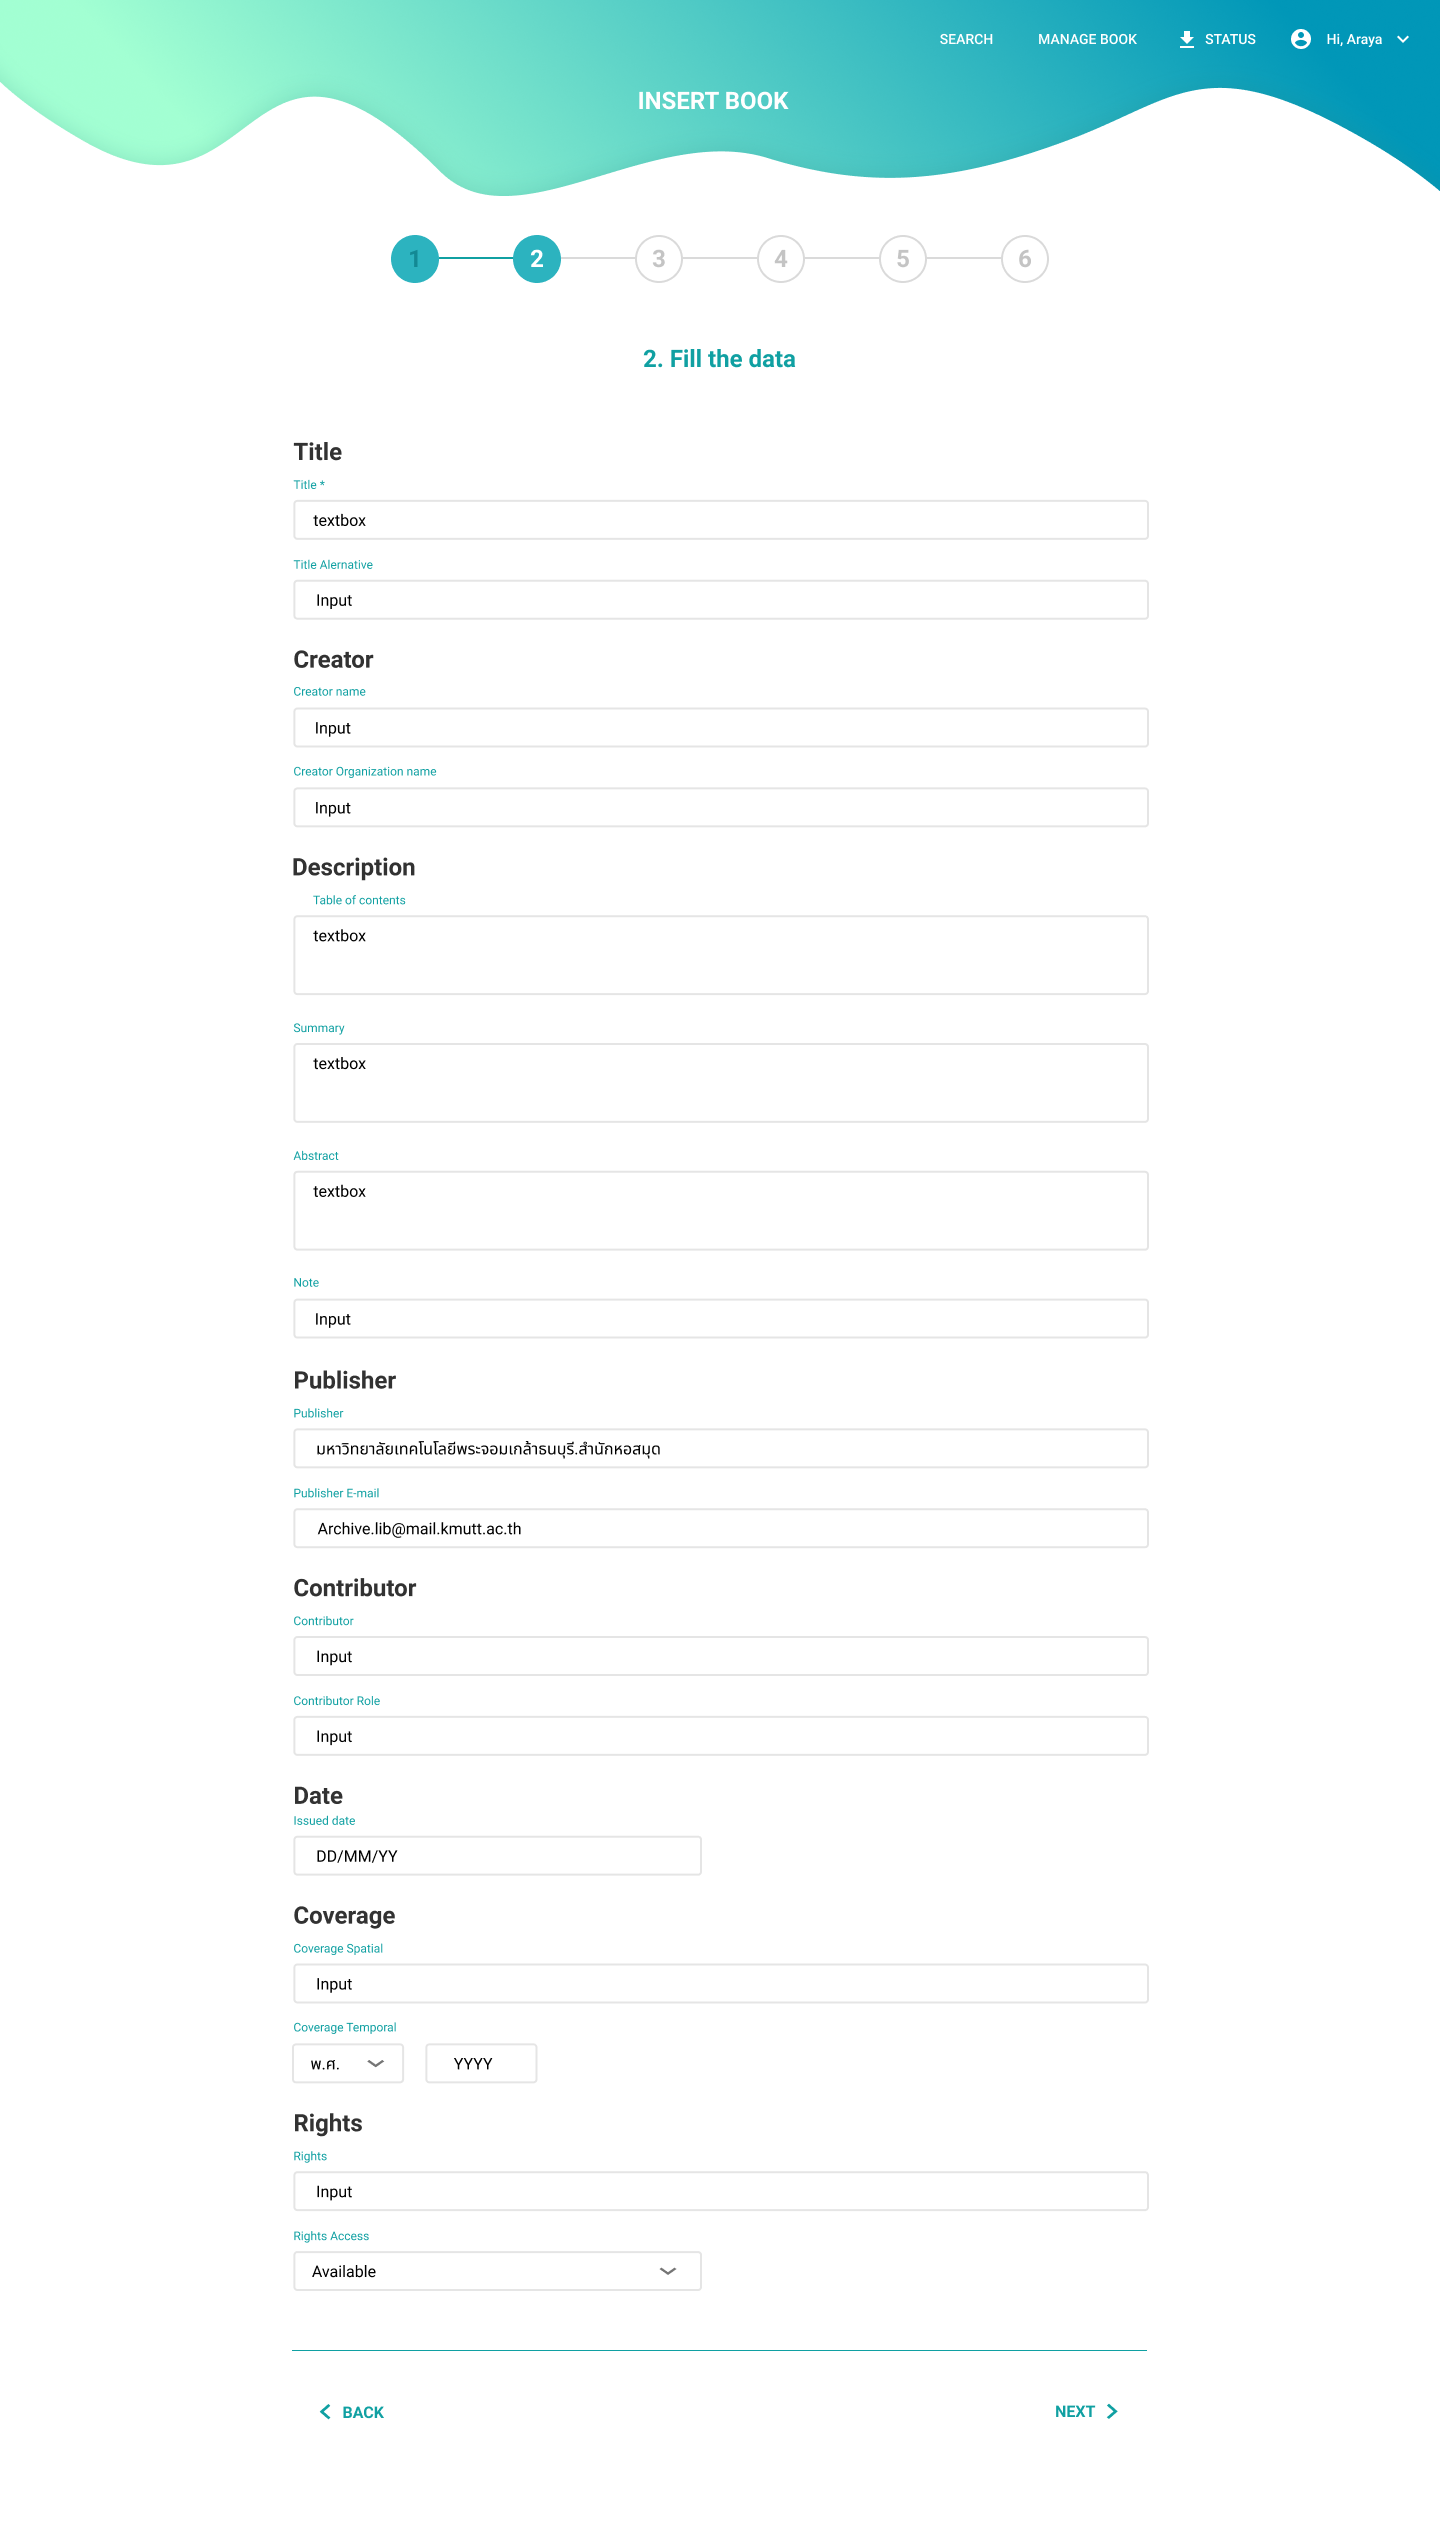
\includegraphics[scale=0.15]{i2}
    \caption{ภาพแสดงขั้นตอนการเพิ่มหนังสือเข้าสู่ระบบขั้นกรอกข้อมูลขั้นที่ 1}\label{fig:i2}
\end{figure}
หน้าเพิ่มหนังสือขั้นตอนที่ 2 เป็นหน้าที่ต้องใส่ข้อมูลที่จำเป็นของหนังสือ โดยที่จำเป็นต้องใส่จะมีสัญลักษณ์กำกับไว้หรือก็คือชื่อหนังสือดังรูป 3.27 โดยในหน้านี้จะมีกล่องใส่ข้อมูลที่ถูกกรอกบ่อย ๆสำหรับผู้ใช้(เจ้าหน้าที่)

\subsection{Insert Book (3)}
\begin{figure}[H]
    \centering
    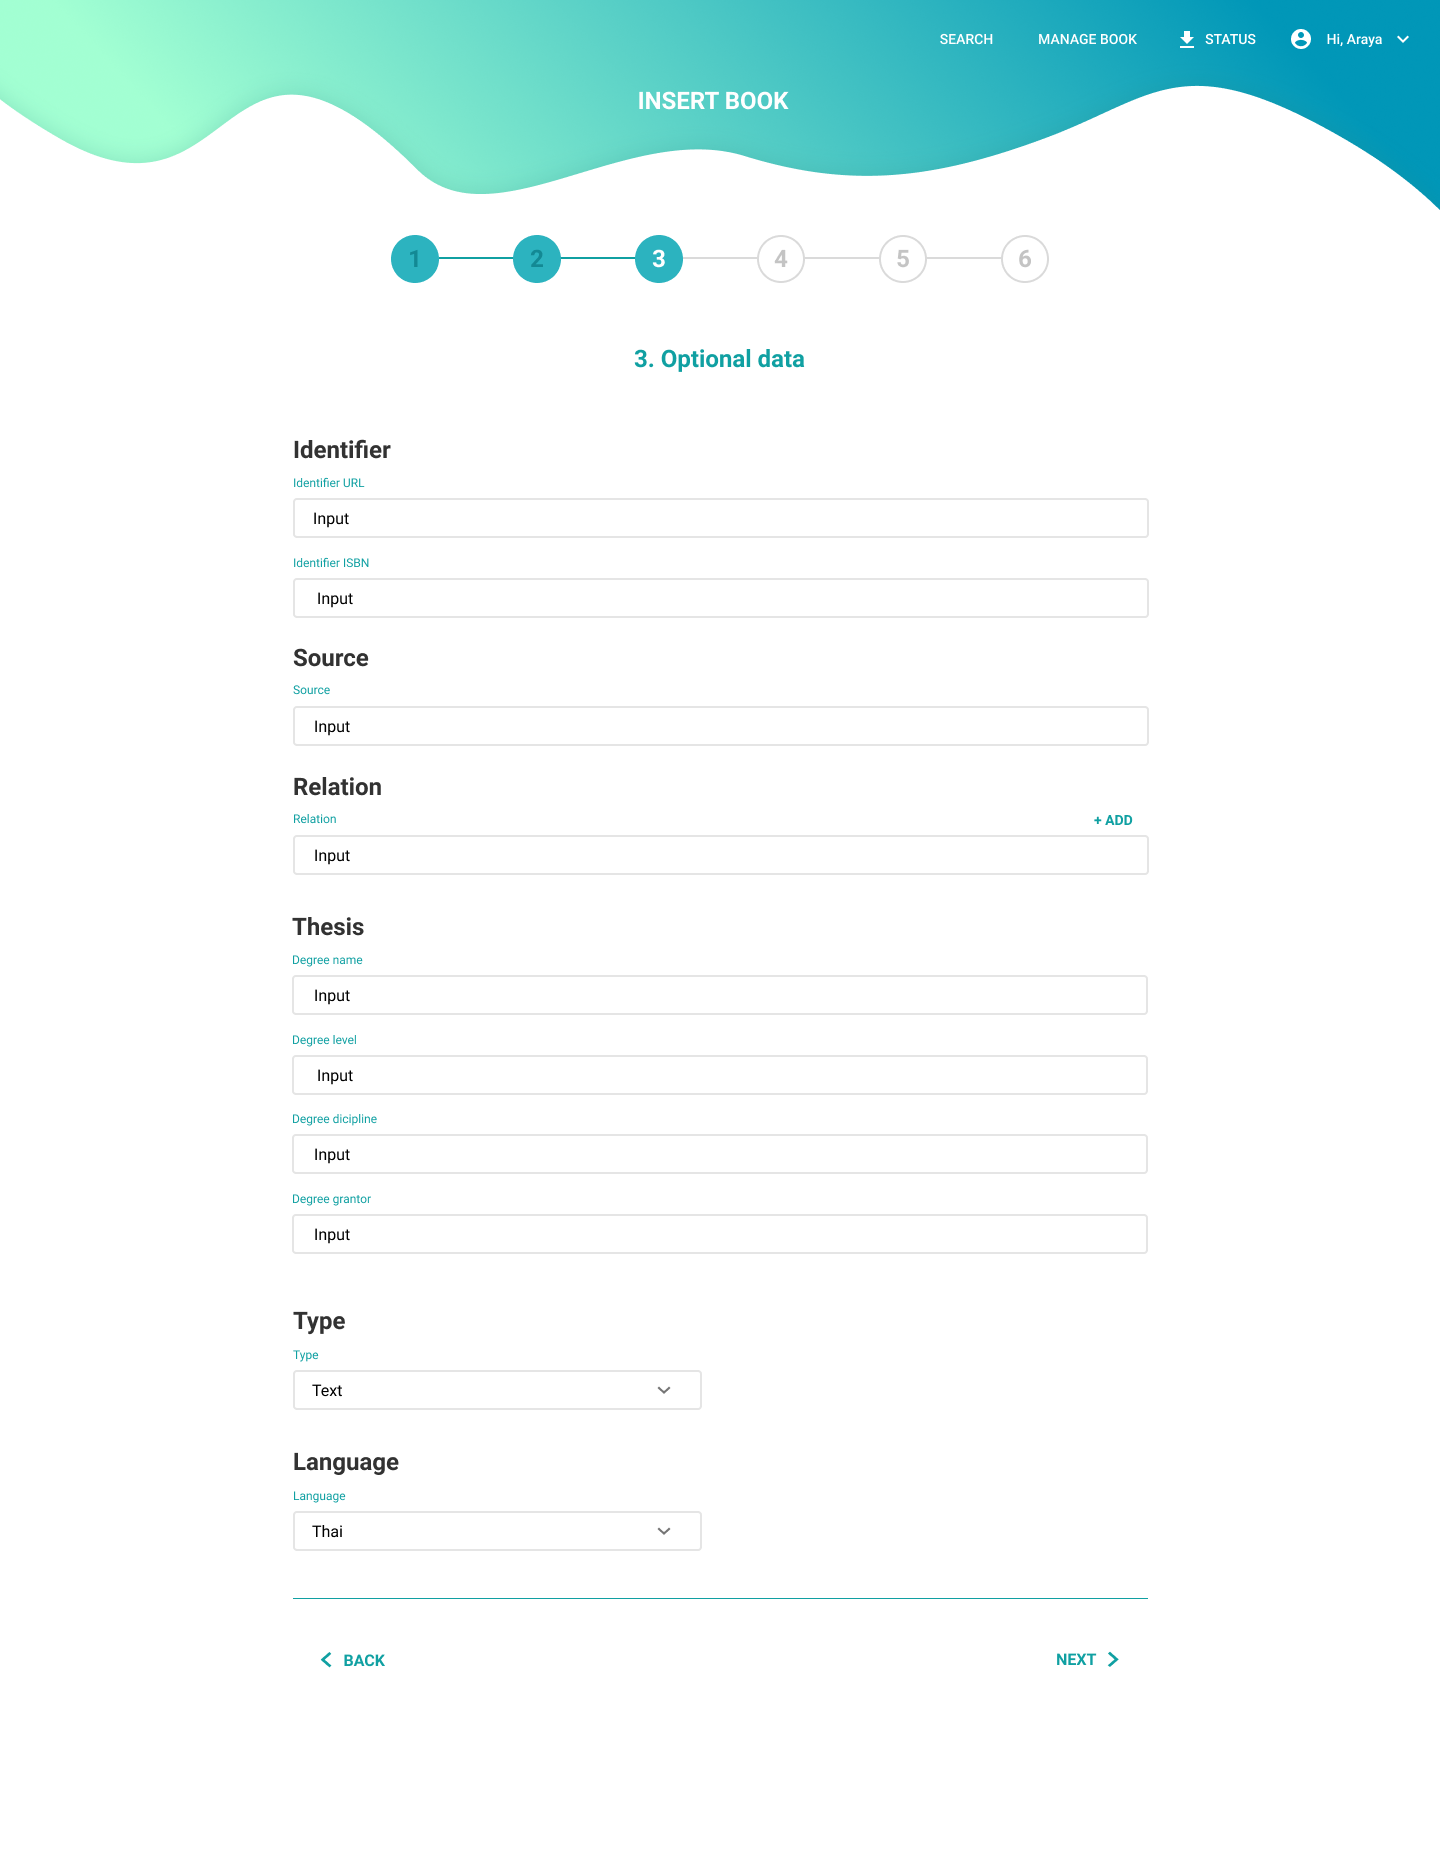
\includegraphics[scale=0.3]{i3}
    \caption{ภาพแสดงขั้นตอนการเพิ่มหนังสือเข้าสู่ระบบขั้นกรอกข้อมูลขั้นที่ 2}\label{fig:i3}
\end{figure}
ในขั้นตอนที่ 3 จากรูปที่ 3.28 จะเป็นหน้าที่ใส่ข้อมูลที่ส่วนใหญ่ผู้ใช้จะไม่ค่อยกรอกมากนัก ซึ่งไม่มีกล่องข้อมูลไหนจำเป็นที่ต้องกรอกผู้ใช้สามารถข้ามไปขั้นตอนถัดไปได้เลย

\subsection{Insert Book (4)}
\begin{figure}[H]
    \centering
    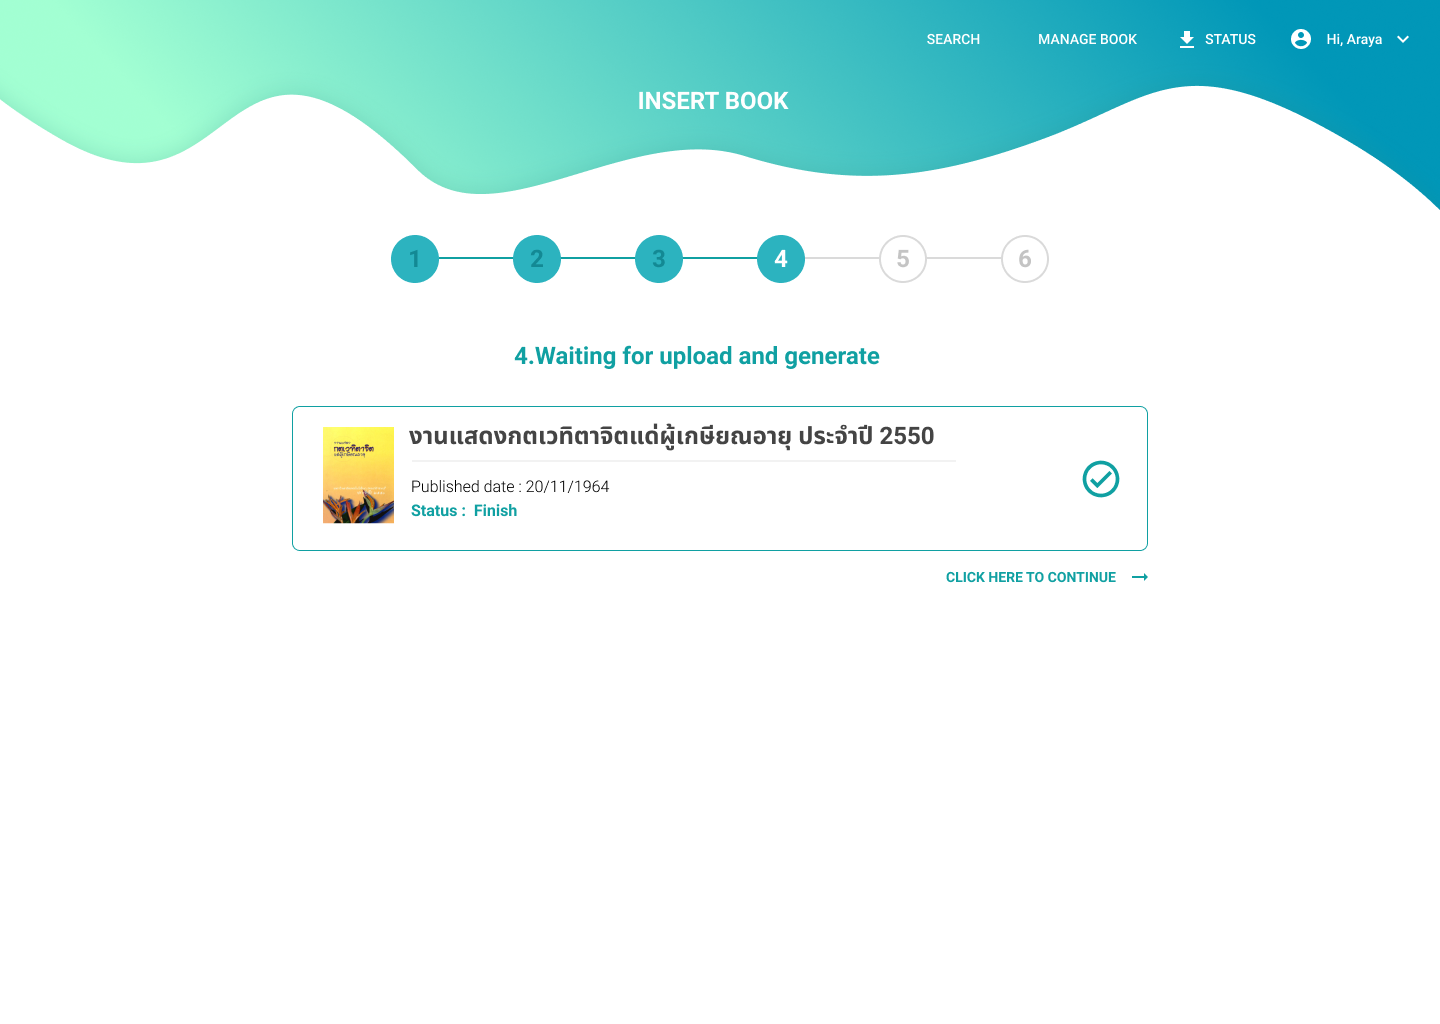
\includegraphics[scale=0.3]{i4}
    \caption{ภาพแสดงขั้นตอนการเพิ่มหนังสือเข้าขั้นโหลดข้อมูลเข้าสู่ระบบ}\label{fig:i4}
\end{figure}
หลังจากที่ทำการใส่ข้อมูลออกมาทั้งหมดแล้วมาถึงหน้าที่เป็นหน้าโหลดข้อมูลดังรูป 3.29 ที่ระบบจะทำการ OCR และทำการเตรียมชุดข้อมูลที่ได้จากการ OCR โดยการนำคำมาตัดและเช็คคำผิด เมื่อโหลดข้อมูลเสร็จแล้วระบบจะทำการเปลี่ยนสถานะการโหลดและขึ้นลิ้งเพื่อเข้าสู่ขั้นตอนถัดไปได้

\subsection{Insert Book (5)}
\begin{figure}[H]
    \centering
    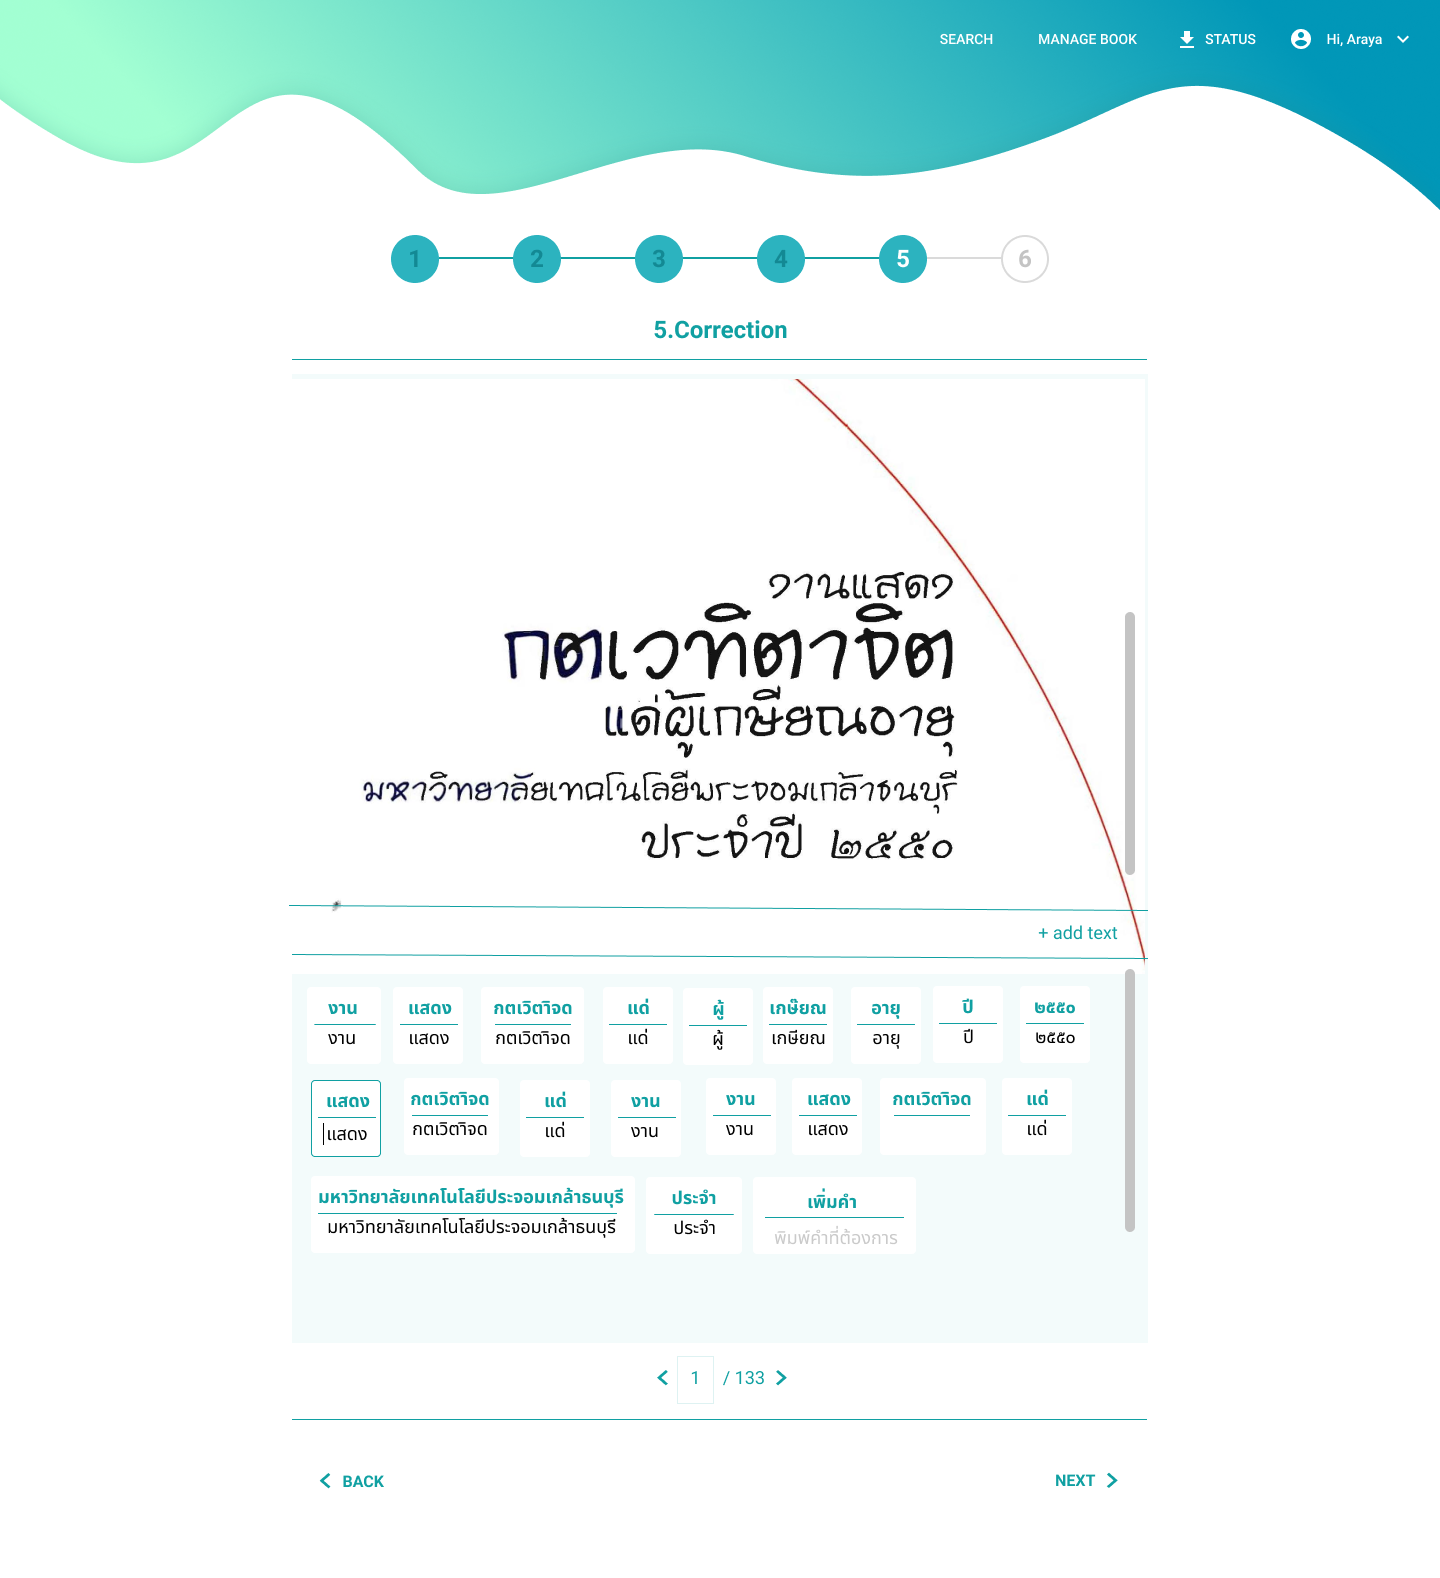
\includegraphics[scale=0.3]{i5}
    \caption{ภาพแสดงขั้นตอนการเพิ่มหนังสือเข้าสู่ระบบขั้นแก้ไขคำผิด}\label{fig:i5}
\end{figure}
หลังจากโหลดและเตรียมข้อมูลเรียบร้อยแล้ว ระบบจะทำการแสดงข้อมูลที่ถูกแปลงมาโดยที่ผู้ใช้จะสามารถแก้ไขคำได้ดังรูป 3.30 หรือสามารถข้ามได้เลยเช่นกัน โดยเมื่อคลิกไปที่กล่องข้อความจะขึ้นให้แก้แต่ละคำและเมื่อเปลี่ยนหน้าจะทำการเก็บข้อมูลที่เปลี่ยนไว้ และจะบันทึกการแก้ไขข้อมูลทั้งหมดที่แก้เมื่อข้ามไปขั้นตอนถัดไป

\subsection{Insert Book (6) }
\begin{figure}[H]
    \centering
    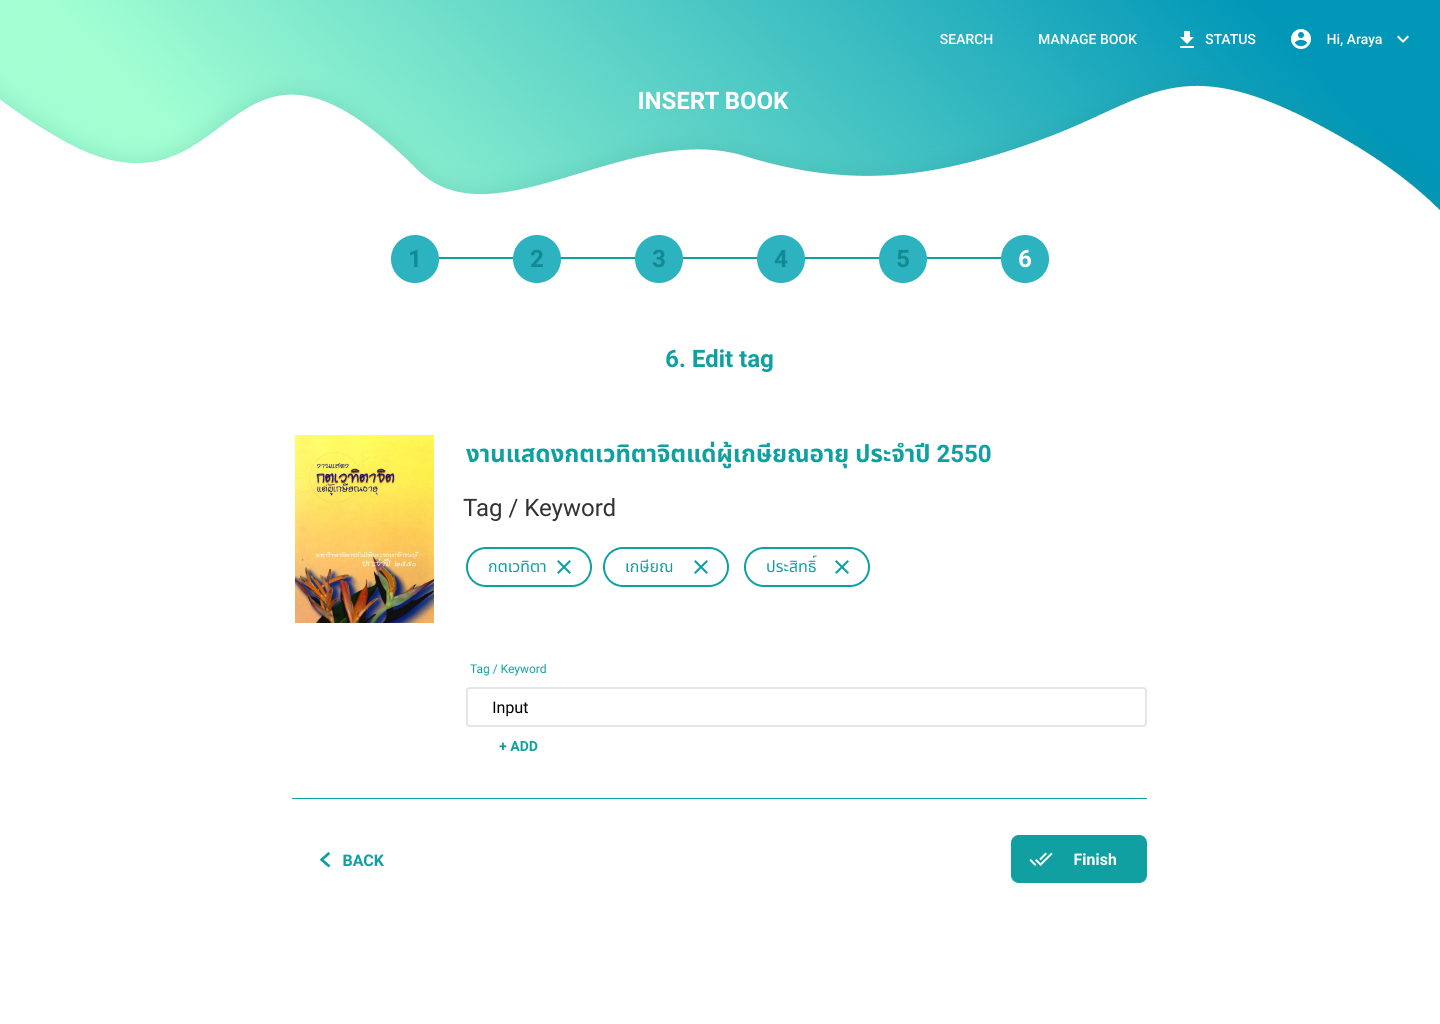
\includegraphics[scale=0.3]{i6}
    \caption{ภาพแสดงขั้นตอนการเพิ่มหนังสือเข้าสู่ระบบขั้นแก้ไขและเพิ่มคำสำคัญ}\label{fig:i6}
\end{figure}
หน้าสุดท้ายของการเพิ่มหนังสือจะเป็นหน้าที่ให้ผู้ใช้สามารถจัดการกับ Keyword ได้ดังรูปที่ 3.31 โดยเมื่อผู้ใช้ต้องการใส่คำสำคัญเพิ่มสามารถกด ADD เพื่อเพิ่มคำที่ต้องการใส่ได้ และสามารถลบเมื่อคลิกที่ปุ่มกากบาทที่คำสำคัญที่ระบบทำการสร้างมาให้ เมื่อแก้ไขเสร็จแล้วสามารถกดปุ่ม Finish เพื่อทำการบันทึกข้อมูล

\subsection{Search}
\begin{figure}[H]
    \centering
    \includegraphics[scale=0.3]{search}
    \caption{ภาพแสดงหน้าค้นหาข้อมูล}\label{fig:search}
\end{figure}
หน้าแสดงข้อมูลการค้นหาเมื่อทำการค้นหาข้อมูลจากหน้าแรก (รูปที่ 3.23 หรือ 3.24) จะทำการแสดงข้อมูลหนังสือที่ตรงกับ keyword โดยเรียงคะแนนของหนังสือที่เกี่ยวข้องกับคำค้นหามากที่สุดดังรูปที่ 3.32 เมื่อกดเข้าไปที่รายชื่อหนังสือจะทำการนำทางผู้ใช้ไปยังหน้าดูหนังสือดังรูปที่ 3.33

\subsection{Document View}
\begin{figure}[H]
    \centering
    \includegraphics[scale=0.3]{lookupp}
    \caption{ภาพแสดงหน้าดูหนังสือ}\label{fig:lookupp}
\end{figure}
เมื่อเราค้นหาและเลือกหนังสือ ก็จะมีหน้าหนังสือ (รูปที่ 3.33) ขึ้นมาให้ดูเนื้อหาภายในโดยที่ผู้ใช้สามารถปรับขนาดภาพและสามารถเลือกหน้าที่ต้องการจะเปิดได้และสามารถย้อนหลับไปยังหน้าเสริชได้ที่ปุ่มลูกศรทางด้านซ้ายบน

\subsection{Manage book}
\begin{figure}[H]
    \centering
    \includegraphics[scale=0.3]{man1}
    \caption{ภาพแสดงหน้าการจัดการหนังสือที่เพิ่มเข้าสู่ระบบ}\label{fig:man1}
\end{figure}
ในหน้าของการจัดการหนังสือดังรูปที่ 3.34 จะมีลักษณะคล้ายกับหน้าการค้นหาเพียงแต่ว่าจะมีฟังก์ชั่นสำหรับการแก้ไขเนื้อหนังสือภายในที่ผู้ใช้เคยกรอกไว้ตอน OCR หนังสือมา เมื่อกดปุ่มลบจะมีหน้าต่างแจ้งเตือนเพื่อถามความแน่ใจในการลบหนังสือ หรือกดปุ่ม Edit เพื่อทำการเข้าสู่การแก้ไขข้อมูลของหนังสือนั้นๆดังรูปที่ 3.35 - 3.37

\subsection{Edit Book}
\begin{figure}[H]
    \centering
    \includegraphics[scale=0.15]{e1}
    \caption{ภาพแสดงขั้นตอนการแก้ไขหนังสือขั้นที่ 1}\label{fig:e1}
\end{figure}

\begin{figure}[H]
    \centering
    \includegraphics[scale=0.3]{e2}
    \caption{ภาพแสดงขั้นตอนการแก้ไขหนังสือขั้นที่ 2}\label{fig:e2}
\end{figure}

\begin{figure}[H]
    \centering
    \includegraphics[scale=0.3]{e3}
    \caption{ภาพแสดงขั้นตอนการแก้ไขหนังสือขั้นที่ 3}\label{fig:e3}
\end{figure}

หน้าแก้ไขหนังสือแบ่งออกเป็น 3 ขั้นตอนดังรูป 3.35 - 3.37 ซึ่งจะมีให้แก้ไข ข้อมูลที่เคยกรอกไว้ตอนเพิ่มหนังสือเข้ามา โดยจะมีรูปปกหนังสือและชื่อหนังสือคอยบอกว่ากำลังแก้ไขหนังสือเล่มไหนอยู่ และในทุกหน้าจะมีปุ่มสำหรับบันทึกในทุกหน้าเพื่อที่จะสามารถบันทึกโดยที่ไม่ต้องรอไปหน้าสุดท้ายเพื่อบันทึกข้อมูล

\subsection{Upload Status Page}
\begin{figure}[H]
    \centering
    \includegraphics[scale=0.3]{status}
    \caption{ภาพแสดงหน้าการโหลดข้อมูล}\label{fig:status}
\end{figure}
จากรูป 3.38 สำหรับผู้ใช้ที่ทำการเพิ่มหนังสือเข้าสู่ระบบจะมีหน้าสำหรับโหลดกรณีที่กดออกมาหลังจากผ่านขั้นตอนการเพิ่มหนังสือขั้นตอนที่ 4 จะสามารถเข้ามาดูสถานะและทำการดำเนินการต่อได้โดยไม่ต้องผ่านการเพิ่มหนังสือเข้าสู่ระบบใหม่


\subsection{Evaluate Process Design}

ในส่วนของการประเมินผลการทำงานนั้นจะแบ่งออกเป็น 3 ส่วนคือการออกแบบ User Interface ส่วนของการเตรียมข้อมูลรูปภาพ จะช่วยให้การทำ OCR มีประสิทธิภาพมากเท่าไร และส่วนของระบบการค้นหา โดยในส่วนของ OCR จะทำการประเมินจากการเลือกเช็คคำจาก 2 หน้าของแต่ละหนังสือมาเช็คว่าแต่ละหน้ามีคำผิดเท่าไร โดยจะเลือกวัดหนังสือทั้งหมด 5 เล่มแบบสุ่มและเทียบการเตรียมข้อมูลรูปภาพ ว่าทำแบบไหนได้ผลลัพธ์แบบไหนออกมา

\begin{table}[H]
\caption{ตารางประเมินการทำ OCR}\label{tbl:ocr}
\begin{tabular}{|c|c|c|c|c|}
\hline
\multicolumn{5}{|c|}{ตารางประเมินการทำ OCR}                 \\ \hline
หนังสือ & หน้า & จำนวนคำทั้งหมด & คำที่ผิด(\%) & คำเกิน(คำ) \\ \hline
        &      &                &              &            \\ \hline
\end{tabular}
\end{table}

ระบบการค้นหา จะเช็คโดยให้ผู้ใช้เป็นผู้ประเมินว่าได้รับหนังสือตรงตามที่ต้องการหรือไม่โดยจะให้เจ้าหน้าที่บรรณารักษ์คัดเลือกหนังสือจำนวน 3 เล่มที่คาดหวังว่าจะขึ้นมาเมื่อค้นหาทั้งหมด 10 ครั้ง

\begin{table}[H]
\caption{ตารางประเมินระบบการค้นหา}\label{tbl:searchtest}
\begin{tabular}{|c|l|p{0.40\linewidth}|}
\hline
\multicolumn{3}{|c|}{ตารางประเมินระบบการค้นหา}                                                                                                                                                                                                                                                                                                                                                                                                                                                                                                                                                \\ \hline
คำค้นหา                & \multicolumn{1}{c|}{หนังสือที่คาดหวัง} & \multicolumn{1}{c|}{การค้นหา}                                                                                                                                                                                                                                                                                                                                                                                                                                                                                               \\ \hline
\multicolumn{1}{|l|}{} &                                        & \makecell[l]{คะแนน 5 ระดับ\\ 5   = ค้นหาหนังสือได้ตรงตามที่ต้องการ \\และมีหนังสือที่เกี่ยวข้องกับคำค้นหาขึ้นมาอย่างถูกต้อง\\ 4   = ค้นหาหนังสือได้ถูกต้องตามที่ต้องการ\\บางเล่มและมีหนังสือที่เกี่ยวข้องกับคำค้นหาขึ้นมา\\ 3   = ไม่สามารถค้นหาหนังสือที่ต้องการแต่\\มีหนังสือที่เกี่ยวข้องกับคำค้นหาขึ้นมา\\ 2   = สามารถค้นหาหนังสือที่มีความเกี่ยวข้องกับคำค้นหา \\และมีหนังสือที่ไม่เกี่ยวข้องกับการค้นหาแสดงในผลัพธ์\\ 1 = ไม่มีหนังสือที่เกี่ยวข้องขึ้นมาในผลลัพธ์} \\ \hline
\end{tabular}
\end{table}

\begin{table}[H]
\caption{ตารางประเมินความพึงพอใจการออกแบบ UX/UI}\label{tbl:uxuieva}
\begin{tabular}{|p{0.15\linewidth}|p{0.15\linewidth}|p{0.15\linewidth}|p{0.15\linewidth}|p{0.15\linewidth}|c|}
\hline
\multicolumn{6}{|c|}{ตารางประเมินการออกแบบ UX/UI}                                                                                                                                                            \\ \hline

                     & \multicolumn{1}{c|}{4}                                                                                                 & \multicolumn{1}{c|}{3}                                                                                   & \multicolumn{1}{c|}{2}                                                                                        & \multicolumn{1}{c|}{1}                                                                        & คะแนนที่ได้ \\ \hline
ความสมบูรณ์ของข้อมูล    & ข้อมูลมีความสมบูรณ์   ชัดเจนทำให้เข้าใจความหมายที่ต้องการจะสื่อได้เป็นอย่างดี                                          & มีข้อมูลที่ชัดเจน   และแม่นยำในบางครั้ง และสามารถแสดงความหมายที่ต้องการจะสื่อได้บ้าง                     & ข้อมูลมีความแม่นยำ   และชัดเจนบ้าง                                                                            & มีข้อมูลที่ไม่ชัดเจน   ไม่ครบ สื่อความหมายได้ไม่ดี                                            &           \\ \hline
การออกแบบ            & มีการออกแบบที่เน้นความสำคัญและจัดวางองค์ประกอบ สี เสียง และการเคลื่อนไหว(animation) ได้อย่างเหมาะสม                                & มีการจัดหน้า   และองค์ประกอบทำให้เห็นใจความสำคัญของเนื้อหา มีการใช้การเคลื่อนไหว(animation)   บ้าง                     & การวางหน้าและการจัดองค์ประกอบมีความไม่เหมาะสม   มีการใช้การเคลื่อนไหว(animation) เข้ามาช่วยบ้าง                             & การวางหน้าและการจัดองค์ประกอบมีความไม่เหมาะสมและไม่มีการใช้  การเคลื่อนไหว(animation) เข้ามาช่วยในการใช้งาน &            \\ \hline
การใช้งาน              & ผู้ใช้สามารถใช้งานปุ่มหรือย้ายไปยังหน้าต่างๆได้อย่างง่ายดาย   แต่มีลิ้งค์ที่พาไปผิดหน้าอย่างมากหนึ่งลิ้งค์หรือไม่มีเลย & ผู้ใช้สามารถใช้งานปุ่มหรือย้ายไปยังหน้าต่างๆได้อย่างง่ายดาย   แต่มีลิ้งค์ที่พาไปผิดหน้าอย่างมากสองลิ้งค์ & ผู้ใช้มีความสับสนในการใช้ปุ่ม   หรือการย้ายไปยังหน้าต่างๆ บางครั้ง และมีลิ้งค์ที่พาไปผิดหน้าอย่างมากสามลิ้งค์ & ผู้ใช้เกิดความสับสนในปุ่มหรือลิ้งค์ที่ย้ายไปหน้าต่างๆ                                         &            \\ \hline
การใช้ภาษา            & มีการใช้คำผิดหรือภาษาที่ไม่เหมาะสมอย่างมาก   1 จุด                                                                     & มีการใช้คำผิดหรือภาษาที่ไม่เหมาะสมอย่างมาก   2 จุด                                                       & มีการใช้คำผิดหรือภาษาที่ไม่เหมาะสมอย่างมาก 3 จุด                                                              & มีการใช้คำผิดหรือภาษาที่ไม่เหมาะสมมากกว่า 4 จุด                                               &            \\ \hline
\end{tabular}
\end{table}
\begin{table}[H]
\caption{ตารางประเมินการทำสอบเว็บไซต์}\label{tbl:test}
\begin{tabular}{|l|l|l|l|}
\hline
\multicolumn{4}{|c|}{ตารางประเมินเว็บไซต์}                                                                                                                                             \\ \hline
\multicolumn{1}{|c|}{\multirow{2}{*}{เกณฑ์การประเมิน}}                  & \multicolumn{2}{c|}{ผลลัพธ์}                             & \multicolumn{1}{c|}{\multirow{2}{*}{หมายเหตุ}} \\ \cline{2-3}
\multicolumn{1}{|c|}{}                                                  & \multicolumn{1}{c|}{ผ่าน} & \multicolumn{1}{c|}{ไม่ผ่าน} & \multicolumn{1}{c|}{}                          \\ \hline
1. สามารถเข้าสู่ระบบและออกจาก ระบบได้                                   &                           &                              &                                                \\ \hline
2. สามารถเพิ่มหนังสือเข้าสู่ระบบได้                                      &                           &                              &                                                \\ \hline
3. สามารถแก้ไขรายละเอียดหนังสือที่อยู่ในระบบได้                          &                           &                              &                                                \\ \hline
4.   สามารถตรวจสอบและแก้ไขคำที่เพิ่มเข้ามาในระบบในขั้นตอนเพิ่มหนังสือได้ &                           &                              &                                                \\ \hline
5. สามารถลบหนังสือที่อยู่ในระบบได้                                       &                           &                              &                                                \\ \hline
6.   สามารถค้นหาข้อมูลหนังสือภายในระบบได้                                &                           &                              &                                                \\ \hline
7.   สามารถเรียกดูหนังสือที่ต้องการได้                                   &                           &                              &                                                \\ \hline
\end{tabular}
\end{table}